% Options for packages loaded elsewhere
\PassOptionsToPackage{unicode}{hyperref}
\PassOptionsToPackage{hyphens}{url}
\PassOptionsToPackage{dvipsnames,svgnames,x11names}{xcolor}
%
\documentclass[
  letterpaper,
  DIV=11,
  numbers=noendperiod]{scrartcl}

\usepackage{amsmath,amssymb}
\usepackage{lmodern}
\usepackage{iftex}
\ifPDFTeX
  \usepackage[T1]{fontenc}
  \usepackage[utf8]{inputenc}
  \usepackage{textcomp} % provide euro and other symbols
\else % if luatex or xetex
  \usepackage{unicode-math}
  \defaultfontfeatures{Scale=MatchLowercase}
  \defaultfontfeatures[\rmfamily]{Ligatures=TeX,Scale=1}
\fi
% Use upquote if available, for straight quotes in verbatim environments
\IfFileExists{upquote.sty}{\usepackage{upquote}}{}
\IfFileExists{microtype.sty}{% use microtype if available
  \usepackage[]{microtype}
  \UseMicrotypeSet[protrusion]{basicmath} % disable protrusion for tt fonts
}{}
\makeatletter
\@ifundefined{KOMAClassName}{% if non-KOMA class
  \IfFileExists{parskip.sty}{%
    \usepackage{parskip}
  }{% else
    \setlength{\parindent}{0pt}
    \setlength{\parskip}{6pt plus 2pt minus 1pt}}
}{% if KOMA class
  \KOMAoptions{parskip=half}}
\makeatother
\usepackage{xcolor}
\usepackage[normalem]{ulem}
\setlength{\emergencystretch}{3em} % prevent overfull lines
\setcounter{secnumdepth}{-\maxdimen} % remove section numbering
% Make \paragraph and \subparagraph free-standing
\ifx\paragraph\undefined\else
  \let\oldparagraph\paragraph
  \renewcommand{\paragraph}[1]{\oldparagraph{#1}\mbox{}}
\fi
\ifx\subparagraph\undefined\else
  \let\oldsubparagraph\subparagraph
  \renewcommand{\subparagraph}[1]{\oldsubparagraph{#1}\mbox{}}
\fi


\providecommand{\tightlist}{%
  \setlength{\itemsep}{0pt}\setlength{\parskip}{0pt}}\usepackage{longtable,booktabs,array}
\usepackage{calc} % for calculating minipage widths
% Correct order of tables after \paragraph or \subparagraph
\usepackage{etoolbox}
\makeatletter
\patchcmd\longtable{\par}{\if@noskipsec\mbox{}\fi\par}{}{}
\makeatother
% Allow footnotes in longtable head/foot
\IfFileExists{footnotehyper.sty}{\usepackage{footnotehyper}}{\usepackage{footnote}}
\makesavenoteenv{longtable}
\usepackage{graphicx}
\makeatletter
\def\maxwidth{\ifdim\Gin@nat@width>\linewidth\linewidth\else\Gin@nat@width\fi}
\def\maxheight{\ifdim\Gin@nat@height>\textheight\textheight\else\Gin@nat@height\fi}
\makeatother
% Scale images if necessary, so that they will not overflow the page
% margins by default, and it is still possible to overwrite the defaults
% using explicit options in \includegraphics[width, height, ...]{}
\setkeys{Gin}{width=\maxwidth,height=\maxheight,keepaspectratio}
% Set default figure placement to htbp
\makeatletter
\def\fps@figure{htbp}
\makeatother

\usepackage{booktabs}
\usepackage{longtable}
\usepackage{array}
\usepackage{multirow}
\usepackage{wrapfig}
\usepackage{float}
\usepackage{colortbl}
\usepackage{pdflscape}
\usepackage{tabu}
\usepackage{threeparttable}
\usepackage{threeparttablex}
\usepackage[normalem]{ulem}
\usepackage{makecell}
\usepackage{xcolor}
\KOMAoption{captions}{tableheading}
\makeatletter
\makeatother
\makeatletter
\makeatother
\makeatletter
\@ifpackageloaded{caption}{}{\usepackage{caption}}
\AtBeginDocument{%
\ifdefined\contentsname
  \renewcommand*\contentsname{Table of contents}
\else
  \newcommand\contentsname{Table of contents}
\fi
\ifdefined\listfigurename
  \renewcommand*\listfigurename{List of Figures}
\else
  \newcommand\listfigurename{List of Figures}
\fi
\ifdefined\listtablename
  \renewcommand*\listtablename{List of Tables}
\else
  \newcommand\listtablename{List of Tables}
\fi
\ifdefined\figurename
  \renewcommand*\figurename{Figure}
\else
  \newcommand\figurename{Figure}
\fi
\ifdefined\tablename
  \renewcommand*\tablename{Table}
\else
  \newcommand\tablename{Table}
\fi
}
\@ifpackageloaded{float}{}{\usepackage{float}}
\floatstyle{ruled}
\@ifundefined{c@chapter}{\newfloat{codelisting}{h}{lop}}{\newfloat{codelisting}{h}{lop}[chapter]}
\floatname{codelisting}{Listing}
\newcommand*\listoflistings{\listof{codelisting}{List of Listings}}
\makeatother
\makeatletter
\@ifpackageloaded{caption}{}{\usepackage{caption}}
\@ifpackageloaded{subcaption}{}{\usepackage{subcaption}}
\makeatother
\makeatletter
\@ifpackageloaded{tcolorbox}{}{\usepackage[many]{tcolorbox}}
\makeatother
\makeatletter
\@ifundefined{shadecolor}{\definecolor{shadecolor}{rgb}{.97, .97, .97}}
\makeatother
\makeatletter
\makeatother
\ifLuaTeX
  \usepackage{selnolig}  % disable illegal ligatures
\fi
\IfFileExists{bookmark.sty}{\usepackage{bookmark}}{\usepackage{hyperref}}
\IfFileExists{xurl.sty}{\usepackage{xurl}}{} % add URL line breaks if available
\urlstyle{same} % disable monospaced font for URLs
\hypersetup{
  pdftitle={Landscape Indices},
  pdfauthor={Maite},
  colorlinks=true,
  linkcolor={blue},
  filecolor={Maroon},
  citecolor={Blue},
  urlcolor={Blue},
  pdfcreator={LaTeX via pandoc}}

\title{Landscape Indices}
\author{Maite}
\date{}

\begin{document}
\maketitle
\ifdefined\Shaded\renewenvironment{Shaded}{\begin{tcolorbox}[interior hidden, borderline west={3pt}{0pt}{shadecolor}, boxrule=0pt, frame hidden, sharp corners, enhanced, breakable]}{\end{tcolorbox}}\fi

This script explores how to use the ATKIS Basis-DLM data 1:50.000 for
incorporating information on the landscape configuration that might be
relevant for biodiversity of grasslands. I'm using the HAI exploratory's
area within Thüringen for a test run (getting ATKIS for the ALB in BaWü
is difficult, unfortunately).

As measure of taxonomic biodiversity, the \textbf{Shannon-Wiener index}
is used (quantifies variety and evenness of species present): relative
abundance of each species (number of individuals per species/total n),
each species relative abundance is multiplied by its natural logarithm,
all values are summed up and negative of sum taken. Higher values mean
more species present and they are more evenly distributed.

Moreover, to grasp functional diversity, XXX is used as a response.

\hypertarget{hypothesis-on-grassland-biodiversity}{%
\section{Hypothesis on grassland
biodiversity}\label{hypothesis-on-grassland-biodiversity}}

Ideas on what aspects of the landscape patterns might be relevant for
biodiversity of grasslands:

\emph{how to translate into method}

\uline{preliminary results on the hypothesis}

\textbf{Patch metric related hypotheses:}

\begin{itemize}
\item
  \textbf{HP1: Species Area Relationship}: larger islands, larger
  species richness (MacArthur, Wilson 1967)

  I.e. (higher equilibrium (immigration vs extinction) number of
  species) Larger areas contain greater variability of habitats
  -\textgreater{} More niches can be satisfied. Larger areas can support
  larger communities which in turn are less likely to become extinct
  (Mittelbach 2019)

  more grassland specialists on larger patches, plant species richness
  increasing with patch size (Loos et al.~2021)

  \begin{itemize}
  \item
    \emph{size of the patch/field, area of connected grassland (what is
    connected? road / forest / ..)}
  \item
    \uline{not verified} (n=XXX, area= XXX)
  \end{itemize}
\item
  \textbf{HP2: Irregularly shaped patches} contain higher number of
  environmental gradients (Honnay 1999) and higher ratio edge length :
  patch size -\textgreater{} higher effects of adjacent agriculture

  \begin{itemize}
  \item
    \emph{ratio edge length : patch size}

    \begin{itemize}
    \tightlist
    \item
      \emph{is there a correlation between patch complexity and
      grassland history and LUI?}
    \end{itemize}
  \end{itemize}
\item
  \textbf{HP3: Grassland next neighbor}: Higher distance between patches
  leads to reduced biodiversity (reduces migration, higher extinction
  risk, lower recolonization probability)

  \begin{itemize}
  \item
    \emph{nearest grassland neighbor distance}
  \item
    \uline{not verified for now}
  \end{itemize}
\item
  \textbf{HP4: Landscape context matters for biodiversity}

  \begin{itemize}
  \tightlist
  \item
    \emph{percent type of land use in surroundings, especially
    agriculture}
  \end{itemize}
\item
  \textbf{HP4a: Percent arable land:} the more arable land within the
  landscape, the less species richness on the grassland plots (Loos et
  al.~2021) arthropod decline for grassland associated with agriculture
  at landscape scale (Li 2023, Seibold 2019)

  \begin{itemize}
  \item
    \emph{percent arable land within landscape}
  \item
    \uline{not verified for now (n=xxx, area=xxx, \ldots)}
  \end{itemize}
\item
  (?) Availability of \textbf{hedges} (Fukamachi et al.~2011, Cherrill
  et al.~2010)
\end{itemize}

\textbf{Landscape history related hypotheses:}

\begin{itemize}
\item
  \textbf{\emph{Historical}} \textbf{patch size and isolation:} Current
  isolation differs strongly from the isolation which occurred when the
  species richness was formed, because many grasslands disappeared. The
  extinction of species in response to isolation might be delayed by 100
  years or more (extinction debt). Thus, historical isolation might be
  more important in describing current diversity than recent
  isolation.Lindborg \& Eriksson (2004) Pärtel et al.~(2005)

  \begin{itemize}
  \tightlist
  \item
    probably only for discussion
  \end{itemize}
\item
  Older patches show higher biodiversity, younger patches have higher
  nutrient levels if used as agricultural land before (Honnay 1999)

  \begin{itemize}
  \tightlist
  \item
    \emph{Grassland history from time series (???) e.g.~via NDVI time
    series with breaking points?}
  \end{itemize}
\end{itemize}

\textbf{Disturbance related hypothesis:}

\begin{itemize}
\item
  \textbf{HD1: Intermediate Disturbance Hypothesis}:\\
  Species Richness highest when moderate disturbance intensity
  (grazing/mowing) because grazing/mowing have disproportional large
  effect on competitive dominants, gaps are produced where proagules can
  establish (Fox 1979, Leps 1999)

  \begin{itemize}
  \item
    \emph{LUI (germany wide)}
  \item
    intermediate LUI and its components lead to highest biodiversity
  \item
    \uline{not verified for LUI (n=xxx, area=xxx), but for mowing
    (n=xxx, area=xxx, sig=xxx)}
  \end{itemize}
\item
  \textbf{HD2: enhanced productivity} \textbf{-\textgreater{} reduction
  in diversity}; fertilization amplifies differences between relative
  growth rates of neighboring ramets, high nutrient adapted plants will
  out compete others (Pärtel 2002, Sammul 2003) \textbf{LU
  intensification} --\textgreater{} species loss, adverse effects on
  dietary specialists, promoting generalist species, homogenized
  assemblages (Christe 2018) Land use intensification, fertilization
  -\textgreater{} reduction of grassland biodiversity: Severe declines
  in plant species richness have been especially caused by intensive
  fertilization (Gross 2009; Socher 2012) such that even common plant
  species have decreased in abundance at alarming rates (Jansen
  2019).~(Freitag et al.~2021)

  \begin{itemize}
  \tightlist
  \item
    \emph{fertilization data / LUI; Poductivity proxy NDVI}
  \end{itemize}
\item
  \textbf{HD3: Inter-annual variation in land use intensity} enhances
  grassland multidiversity (Allan 2014) especially in rarer species

  \begin{itemize}
  \item
    \emph{LUI temporal variability}
  \item
    \uline{not verified for now (xxx)}
  \end{itemize}
\end{itemize}

\textbf{Abiotic habitat related hypotheses:}

\begin{itemize}
\item
  \textbf{HA1: Habitat heterogeneity hypothesis}: Abiotic diversity
  creates different niches --\textgreater{} higher species richness
  (Burnett 2008, Heidrich 2020)

  probably only important to compare between explos, perhaps Zeigerwerte
  model analysis / discussion

  \begin{itemize}
  \tightlist
  \item
    \emph{SD abiotic predictors (terrain, \ldots) in environment}
  \end{itemize}
\item
  \textbf{HA2: Soil properties are relevant for grassland biodiversity}

  \begin{itemize}
  \tightlist
  \item
    \emph{soil type, bedrock, distance to groundwater, soil
    texture\ldots{}}
  \end{itemize}
\item
  \textbf{HA2a: High pH, higher species richness}: were more abundant
  during evolutionary times at high latitudes (Pärtel 2002)

  \begin{itemize}
  \tightlist
  \item
    \emph{pH}
  \end{itemize}
\item
  \textbf{HA2b: Soil depth} effects on grassland communities and landuse
  practices interact: Soil depth had a strong positive effect on species
  richness under mowing, suggesting increased space for niche
  differentiation in deeper soils. In unmown plots, deep soils harboured
  a similar diversity of species as shallow soils, and our findings
  suggest that this effect on diversity is due to larger biomass and
  lower light availability on deep soils. Fertilization and trampling
  had no effect on diversity. (Braun 2022)~

  \begin{itemize}
  \tightlist
  \item
    \emph{soil depth, mowing frequency}
  \end{itemize}
\end{itemize}

\hypertarget{unify-adjacent-grassland-patches}{%
\subparagraph{Unify adjacent grassland
patches}\label{unify-adjacent-grassland-patches}}

\hypertarget{hp1-grassland-patch-size}{%
\subsubsection{HP1: Grassland patch
size}\label{hp1-grassland-patch-size}}

\hypertarget{calculate-grassland-area-around-patch}{%
\subparagraph{calculate grassland area around
patch}\label{calculate-grassland-area-around-patch}}

The following map shows

\begin{itemize}
\item
  Which grassland geometries contain exploratory plots
\item
  What is the grassland area that surrounds the plots
\end{itemize}

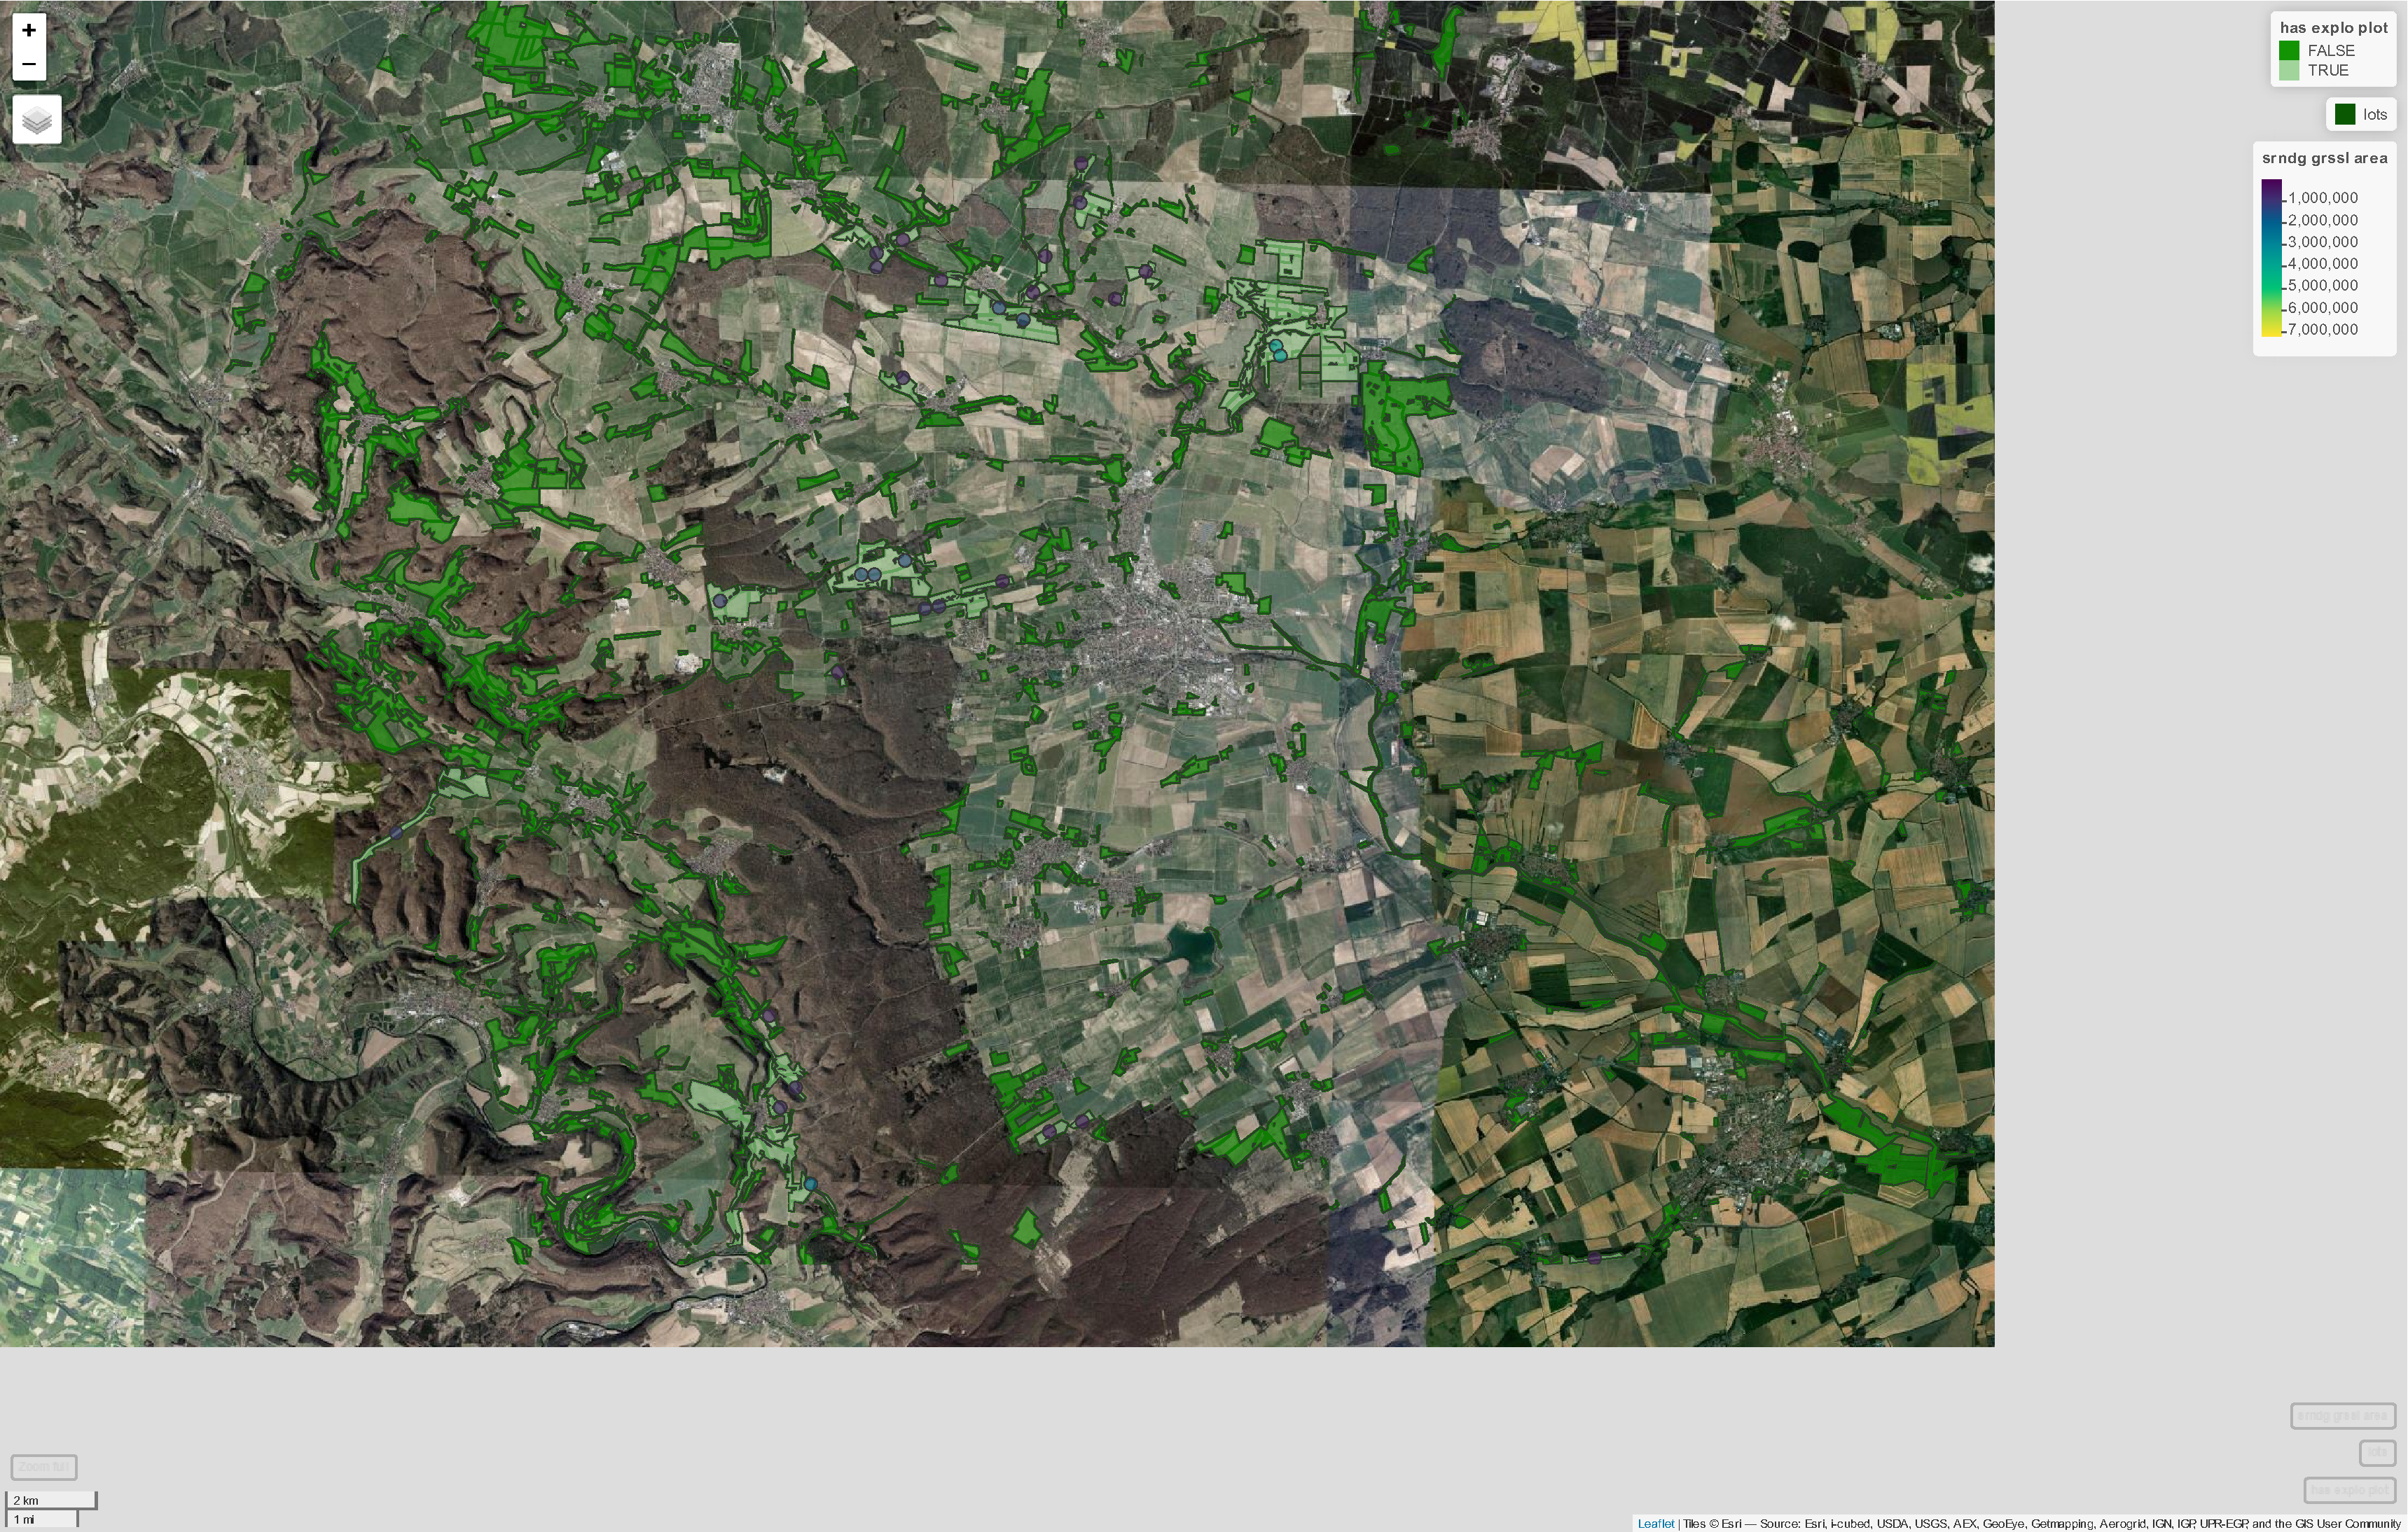
\includegraphics{Landscape_Indices_files/figure-pdf/unnamed-chunk-8-1.pdf}

Just checking: But as anticipated, there is, on its own, no clear
relationship between the grassland area and biodiversity (only from
2013, though, at the time):

\begin{figure}

\begin{minipage}[t]{0.50\linewidth}

{\centering 

\raisebox{-\height}{

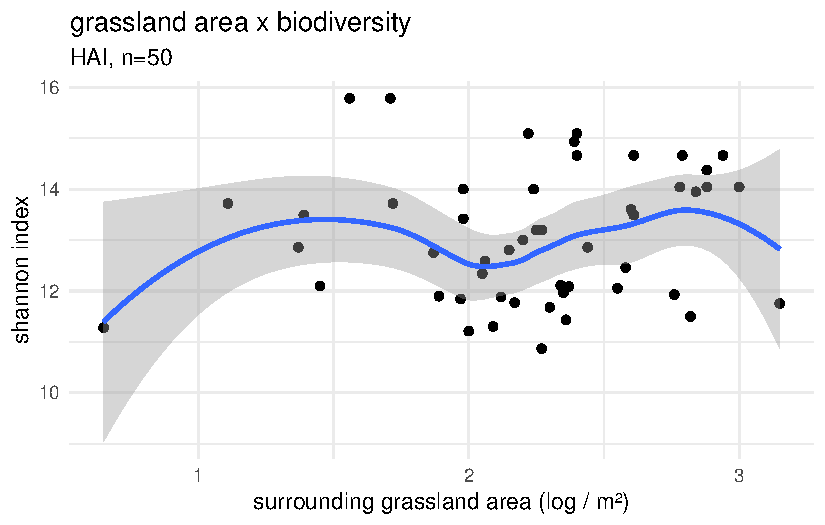
\includegraphics{Landscape_Indices_files/figure-pdf/unnamed-chunk-9-1.pdf}

}

}

\end{minipage}%
%
\begin{minipage}[t]{0.50\linewidth}

{\centering 

\raisebox{-\height}{

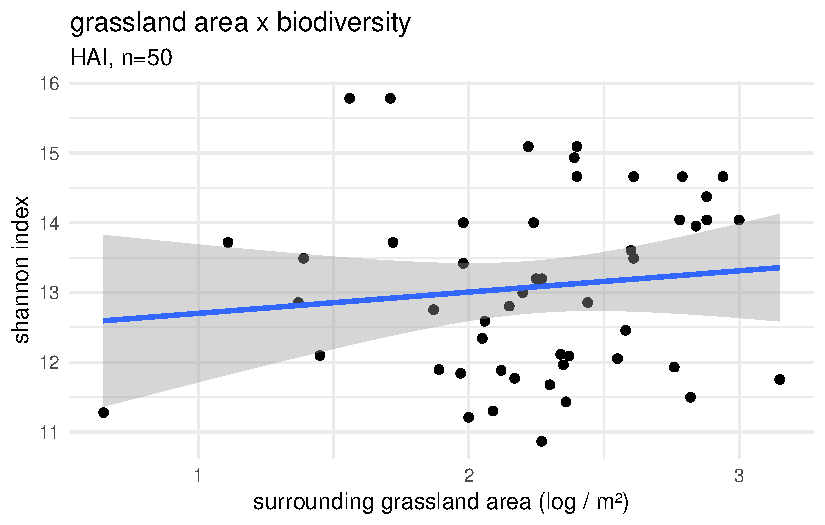
\includegraphics{Landscape_Indices_files/figure-pdf/unnamed-chunk-9-2.pdf}

}

}

\end{minipage}%

\end{figure}

→ HP1: could be, no major evidence, though, from HAI.

\hypertarget{land-use-composition-within-surroundings}{%
\subsubsection{\texorpdfstring{Land use \textbf{composition within
surroundings}}{Land use composition within surroundings}}\label{land-use-composition-within-surroundings}}

\hypertarget{calculate-proportion-of-other-dlm-types}{%
\subparagraph{Calculate proportion of other DLM
types}\label{calculate-proportion-of-other-dlm-types}}

Looking into the proportion of DLM types within a buffer of radius 500m²
surrounding the patch:

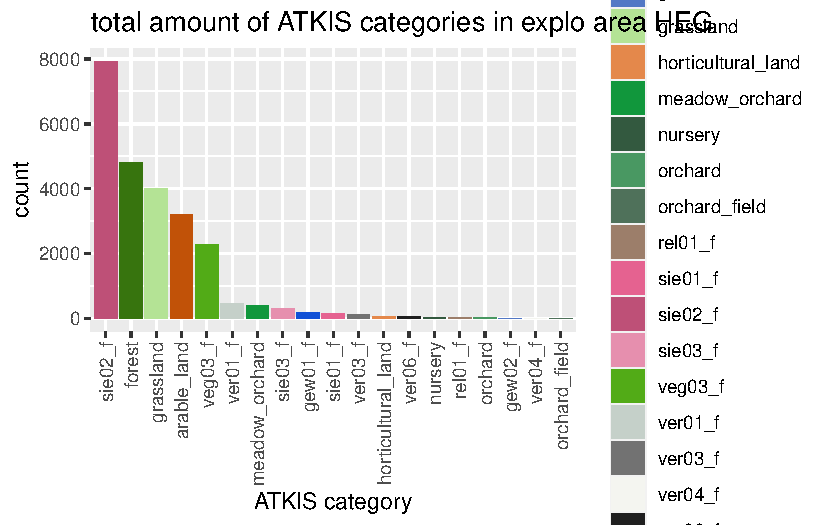
\includegraphics{Landscape_Indices_files/figure-pdf/unnamed-chunk-11-1.pdf}

Work on the categories:

\begin{itemize}
\item
  remove rel01\_f? is it relevant for other areas?
\item
  separate stehendes Gewässer and Fließgewässer (in gew01\_f)
\item
  make something like Teilversiegelt \& Versiegelt from sie01 and sie02
\item
  join categories in veg01? e.g.~orchards and nursery? Not so sure that
  would be a good idea\ldots{} (?)
\item
  what about Sumpf?
\item
  Add Gehölz to Wald?
\item
  Verkehr komplett zu versiegelte Fläche
\end{itemize}

\begin{tabu} to \linewidth {>{\raggedright}X>{\raggedright}X>{\raggedright}X>{\raggedright}X>{\raggedright}X}
\hline
  & rel\_cat & nam & rel\_info & colors\\
\hline
8027 & gew01\_f & gew01\_f & AX\_StehendesGewaesser & \cellcolor[HTML]{1050D6}{\textcolor{white}{\#1050D6}}\\
\hline
8211 & gew01\_f & gew01\_f & AX\_Fliessgewaesser & \cellcolor[HTML]{1050D6}{\textcolor{white}{\#1050D6}}\\
\hline
8227 & gew02\_f & gew02\_f & AX\_Gewaessermerkmal & \cellcolor[HTML]{5378C5}{\textcolor{white}{\#5378C5}}\\
\hline
12786 & rel01\_f & rel01\_f & AX\_FelsenFelsblockFelsnadel & \cellcolor[HTML]{9C7E6A}{\textcolor{white}{\#9C7E6A}}\\
\hline
12819 & sie01\_f & sie01\_f & AX\_Ortslage & \cellcolor[HTML]{E56290}{\textcolor{white}{\#E56290}}\\
\hline
12971 & sie02\_f & sie02\_f & AX\_FlaecheGemischterNutzung & \cellcolor[HTML]{BE5077}{\textcolor{white}{\#BE5077}}\\
\hline
12979 & sie02\_f & sie02\_f & AX\_FlaecheBesondererFunktionalerPraegung & \cellcolor[HTML]{BE5077}{\textcolor{white}{\#BE5077}}\\
\hline
15237 & sie02\_f & sie02\_f & AX\_Friedhof & \cellcolor[HTML]{BE5077}{\textcolor{white}{\#BE5077}}\\
\hline
16827 & sie02\_f & sie02\_f & AX\_IndustrieUndGewerbeflaeche & \cellcolor[HTML]{BE5077}{\textcolor{white}{\#BE5077}}\\
\hline
17123 & sie02\_f & sie02\_f & AX\_Halde & \cellcolor[HTML]{BE5077}{\textcolor{white}{\#BE5077}}\\
\hline
18010 & sie02\_f & sie02\_f & AX\_SportFreizeitUndErholungsflaeche & \cellcolor[HTML]{BE5077}{\textcolor{white}{\#BE5077}}\\
\hline
19262 & sie02\_f & sie02\_f & AX\_TagebauGrubeSteinbruch & \cellcolor[HTML]{BE5077}{\textcolor{white}{\#BE5077}}\\
\hline
19299 & sie02\_f & sie02\_f & AX\_Wohnbauflaeche & \cellcolor[HTML]{BE5077}{\textcolor{white}{\#BE5077}}\\
\hline
20905 & sie03\_f & sie03\_f & AX\_BauwerkOderAnlageFuerSportFreizeitUndErholung & \cellcolor[HTML]{E68FAE}{\textcolor{white}{\#E68FAE}}\\
\hline
20906 & sie03\_f & sie03\_f & AX\_BauwerkOderAnlageFuerIndustrieUndGewerbe & \cellcolor[HTML]{E68FAE}{\textcolor{white}{\#E68FAE}}\\
\hline
21162 & sie03\_f & sie03\_f & AX\_HistorischesBauwerkOderHistorischeEinrichtung & \cellcolor[HTML]{E68FAE}{\textcolor{white}{\#E68FAE}}\\
\hline
21167 & sie03\_f & sie03\_f & AX\_SonstigesBauwerkOderSonstigeEinrichtung & \cellcolor[HTML]{E68FAE}{\textcolor{white}{\#E68FAE}}\\
\hline
21173 & sie03\_f & sie03\_f & AX\_Transportanlage & \cellcolor[HTML]{E68FAE}{\textcolor{white}{\#E68FAE}}\\
\hline
21174 & sie03\_f & sie03\_f & AX\_VorratsbehaelterSpeicherbauwerk & \cellcolor[HTML]{E68FAE}{\textcolor{white}{\#E68FAE}}\\
\hline
1 & arable\_land & veg01\_f & arable\_land & \cellcolor[HTML]{C15208}{\textcolor{white}{\#C15208}}\\
\hline
8235 & grassland & veg01\_f & grassland & \cellcolor[HTML]{B4E395}{\textcolor{white}{\#B4E395}}\\
\hline
12238 & horticultural\_land & veg01\_f & horticultural\_land & \cellcolor[HTML]{E4884B}{\textcolor{white}{\#E4884B}}\\
\hline
12309 & meadow\_orchard & veg01\_f & meadow\_orchard & \cellcolor[HTML]{11973C}{\textcolor{white}{\#11973C}}\\
\hline
12720 & nursery & veg01\_f & nursery & \cellcolor[HTML]{33593F}{\textcolor{white}{\#33593F}}\\
\hline
12760 & orchard & veg01\_f & orchard & \cellcolor[HTML]{499862}{\textcolor{white}{\#499862}}\\
\hline
12783 & orchard\_field & veg01\_f & orchard\_field & \cellcolor[HTML]{4F715A}{\textcolor{white}{\#4F715A}}\\
\hline
3206 & forest & veg02\_f & AX\_Wald & \cellcolor[HTML]{37740E}{\textcolor{white}{\#37740E}}\\
\hline
21217 & veg03\_f & veg03\_f & AX\_Gehoelz & \cellcolor[HTML]{52AB17}{\textcolor{white}{\#52AB17}}\\
\hline
22799 & veg03\_f & veg03\_f & AX\_Heide & \cellcolor[HTML]{52AB17}{\textcolor{white}{\#52AB17}}\\
\hline
22809 & veg03\_f & veg03\_f & AX\_UnlandVegetationsloseFlaeche & \cellcolor[HTML]{52AB17}{\textcolor{white}{\#52AB17}}\\
\hline
22834 & veg03\_f & veg03\_f & AX\_Sumpf & \cellcolor[HTML]{52AB17}{\textcolor{white}{\#52AB17}}\\
\hline
23500 & ver01\_f & ver01\_f & AX\_Platz & \cellcolor[HTML]{C5D0C9}{\textcolor{white}{\#C5D0C9}}\\
\hline
23584 & ver01\_f & ver01\_f & AX\_Strassenverkehr & \cellcolor[HTML]{C5D0C9}{\textcolor{white}{\#C5D0C9}}\\
\hline
23960 & ver03\_f & ver03\_f & AX\_Bahnverkehr & \cellcolor[HTML]{727272}{\textcolor{white}{\#727272}}\\
\hline
24080 & ver04\_f & ver04\_f & AX\_Flugverkehr & \cellcolor[HTML]{F4F5F0}{\textcolor{white}{\#F4F5F0}}\\
\hline
24084 & ver06\_f & ver06\_f & AX\_Bahnverkehrsanlage & \cellcolor[HTML]{1F1F1F}{\textcolor{white}{\#1F1F1F}}\\
\hline
24085 & ver06\_f & ver06\_f & AX\_BauwerkImVerkehrsbereich & \cellcolor[HTML]{1F1F1F}{\textcolor{white}{\#1F1F1F}}\\
\hline
24089 & ver06\_f & ver06\_f & AX\_BauwerkImGewaesserbereich & \cellcolor[HTML]{1F1F1F}{\textcolor{white}{\#1F1F1F}}\\
\hline
24132 & ver06\_f & ver06\_f & AX\_Flugverkehrsanlage & \cellcolor[HTML]{1F1F1F}{\textcolor{white}{\#1F1F1F}}\\
\hline
\end{tabu}

Make a buffer of radius = 500m², i.e.~196.350m² around explo plots and
take a look at proportions of DLM inside the buffer. Veg04
(Vegetationsmerkmale) was eliminated since it caused overlapping.

rel = relief (Felsen / Felsblock)

https://www.adv-online.de/icc/extdeu/nav/a63/binarywriterservlet\%3FimgUid\%3D9201016e-7efa-8461-e336-b6951fa2e0c9\%26uBasVariant\%3D11111111-1111-1111-1111-111111111111

Vegetation categories are as follows:

\includegraphics{ATKIS_vegetation.png}

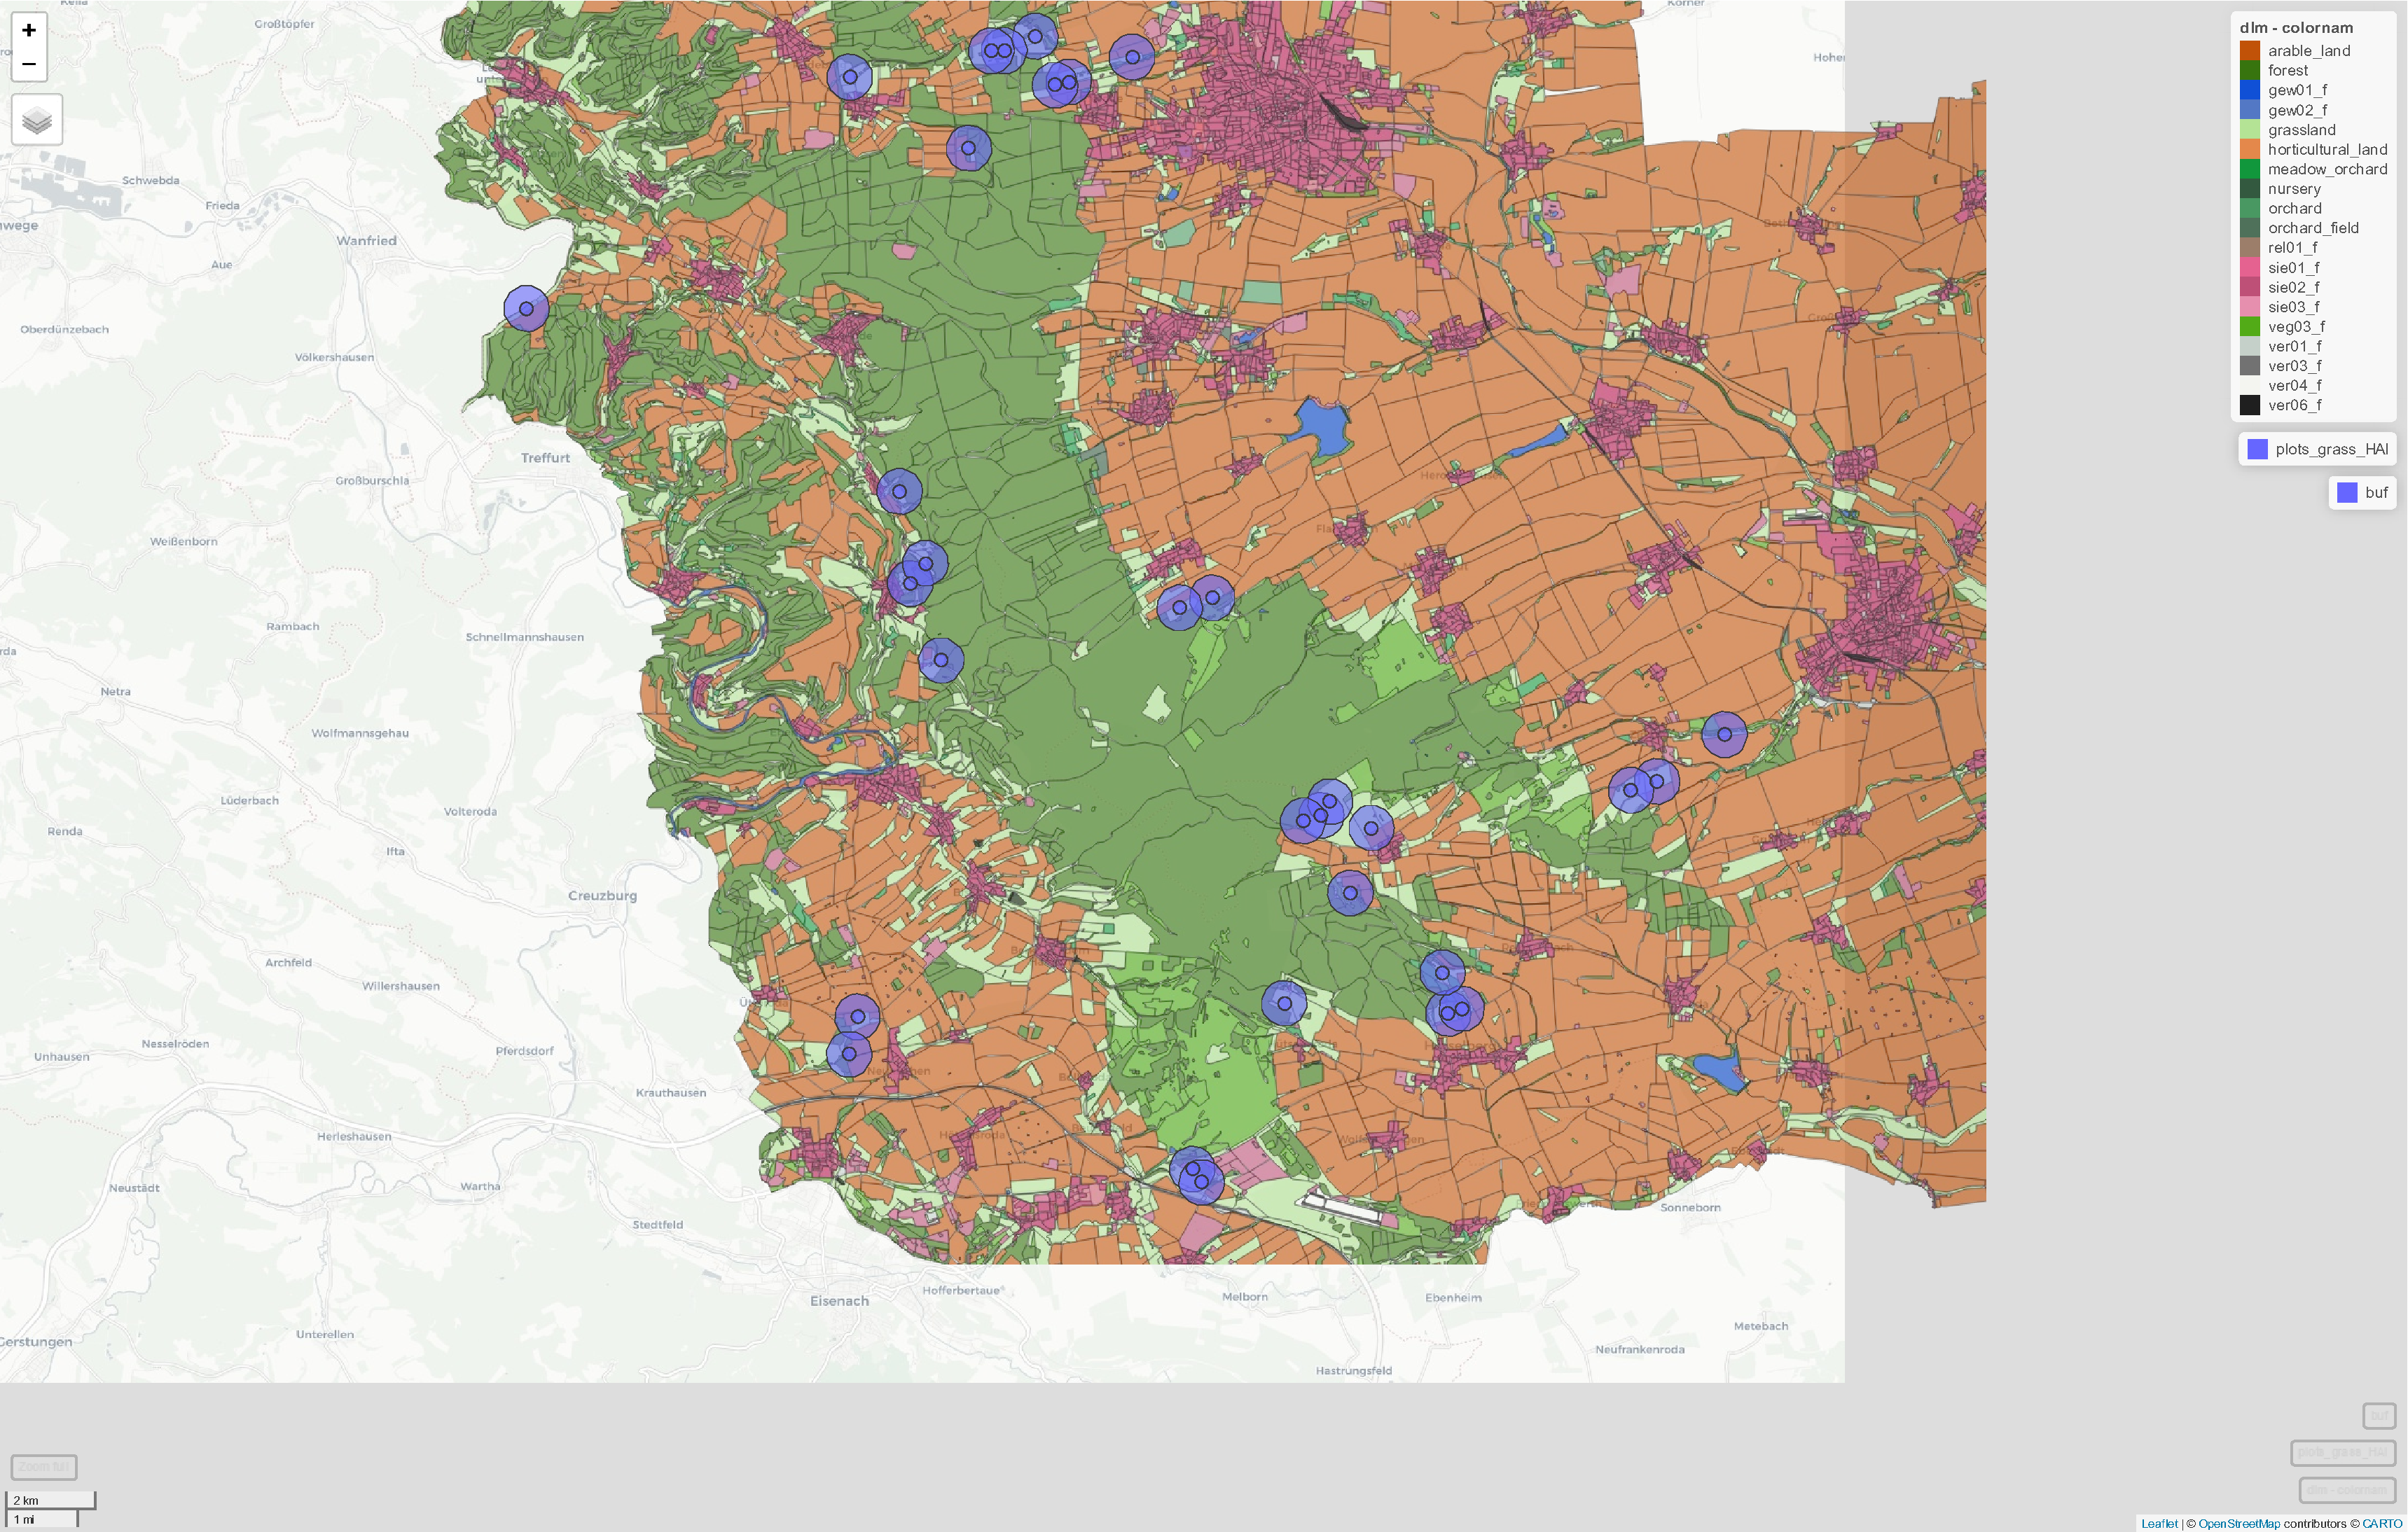
\includegraphics{Landscape_Indices_files/figure-pdf/unnamed-chunk-14-1.pdf}

\hypertarget{exemplary-plots}{%
\subparagraph{exemplary plots}\label{exemplary-plots}}

Maybe sum up Gehölz and Wald into one category? Take a look at northern
plot for this\ldots{}

\begin{verbatim}
[[1]]
\end{verbatim}

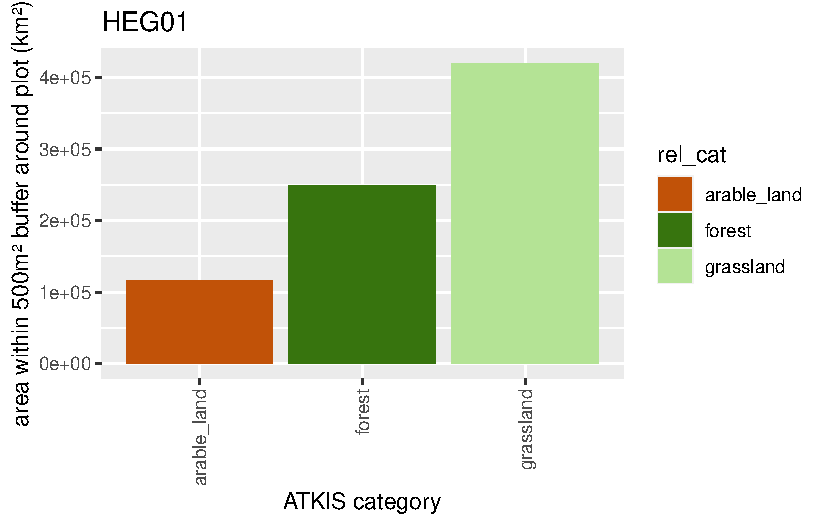
\includegraphics{Landscape_Indices_files/figure-pdf/unnamed-chunk-15-1.pdf}

\begin{verbatim}

[[2]]
\end{verbatim}

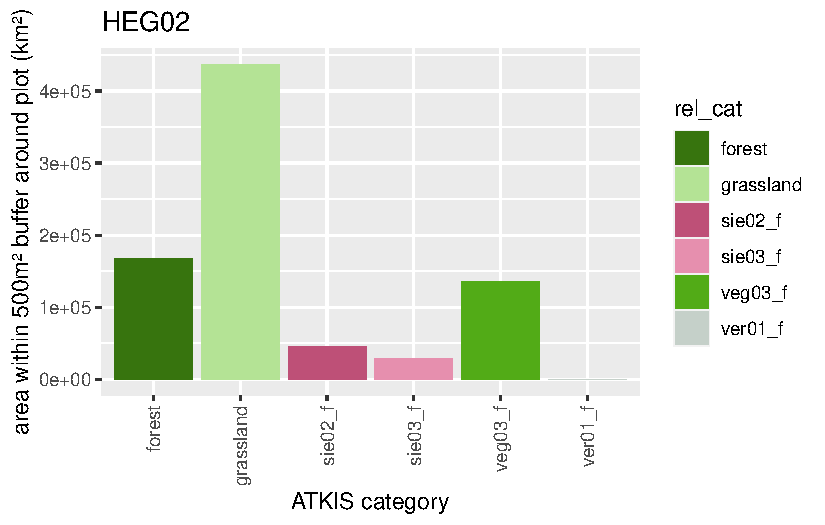
\includegraphics{Landscape_Indices_files/figure-pdf/unnamed-chunk-15-2.pdf}

\begin{verbatim}

[[3]]
\end{verbatim}

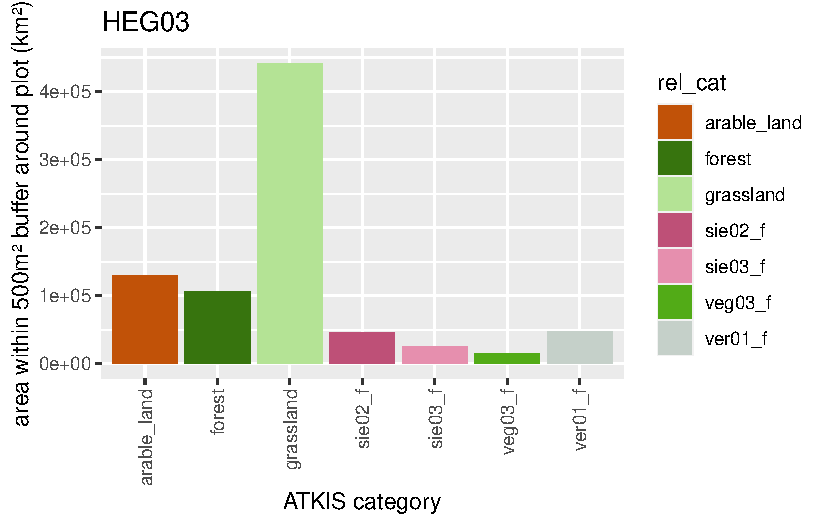
\includegraphics{Landscape_Indices_files/figure-pdf/unnamed-chunk-15-3.pdf}

\begin{verbatim}

[[4]]
\end{verbatim}

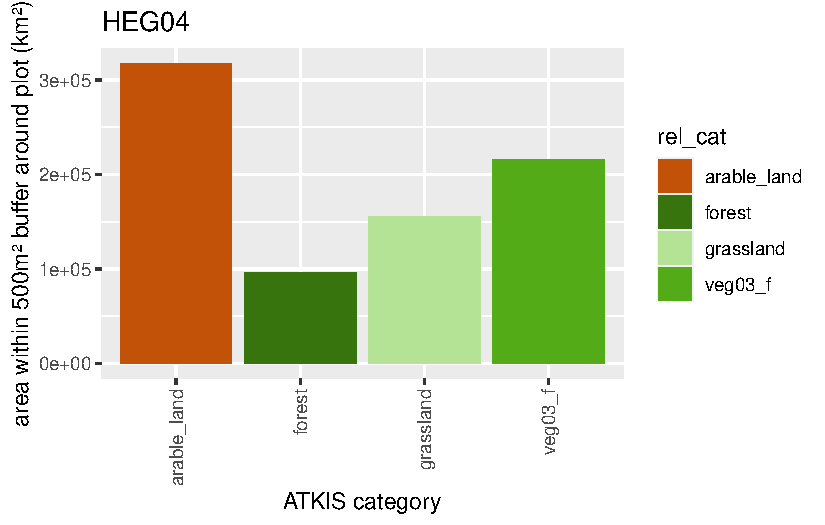
\includegraphics{Landscape_Indices_files/figure-pdf/unnamed-chunk-15-4.pdf}

\begin{verbatim}

[[5]]
\end{verbatim}

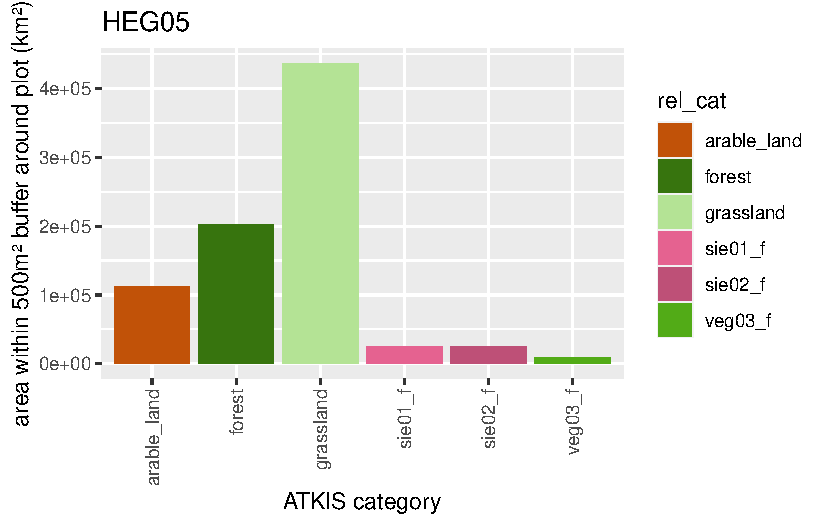
\includegraphics{Landscape_Indices_files/figure-pdf/unnamed-chunk-15-5.pdf}

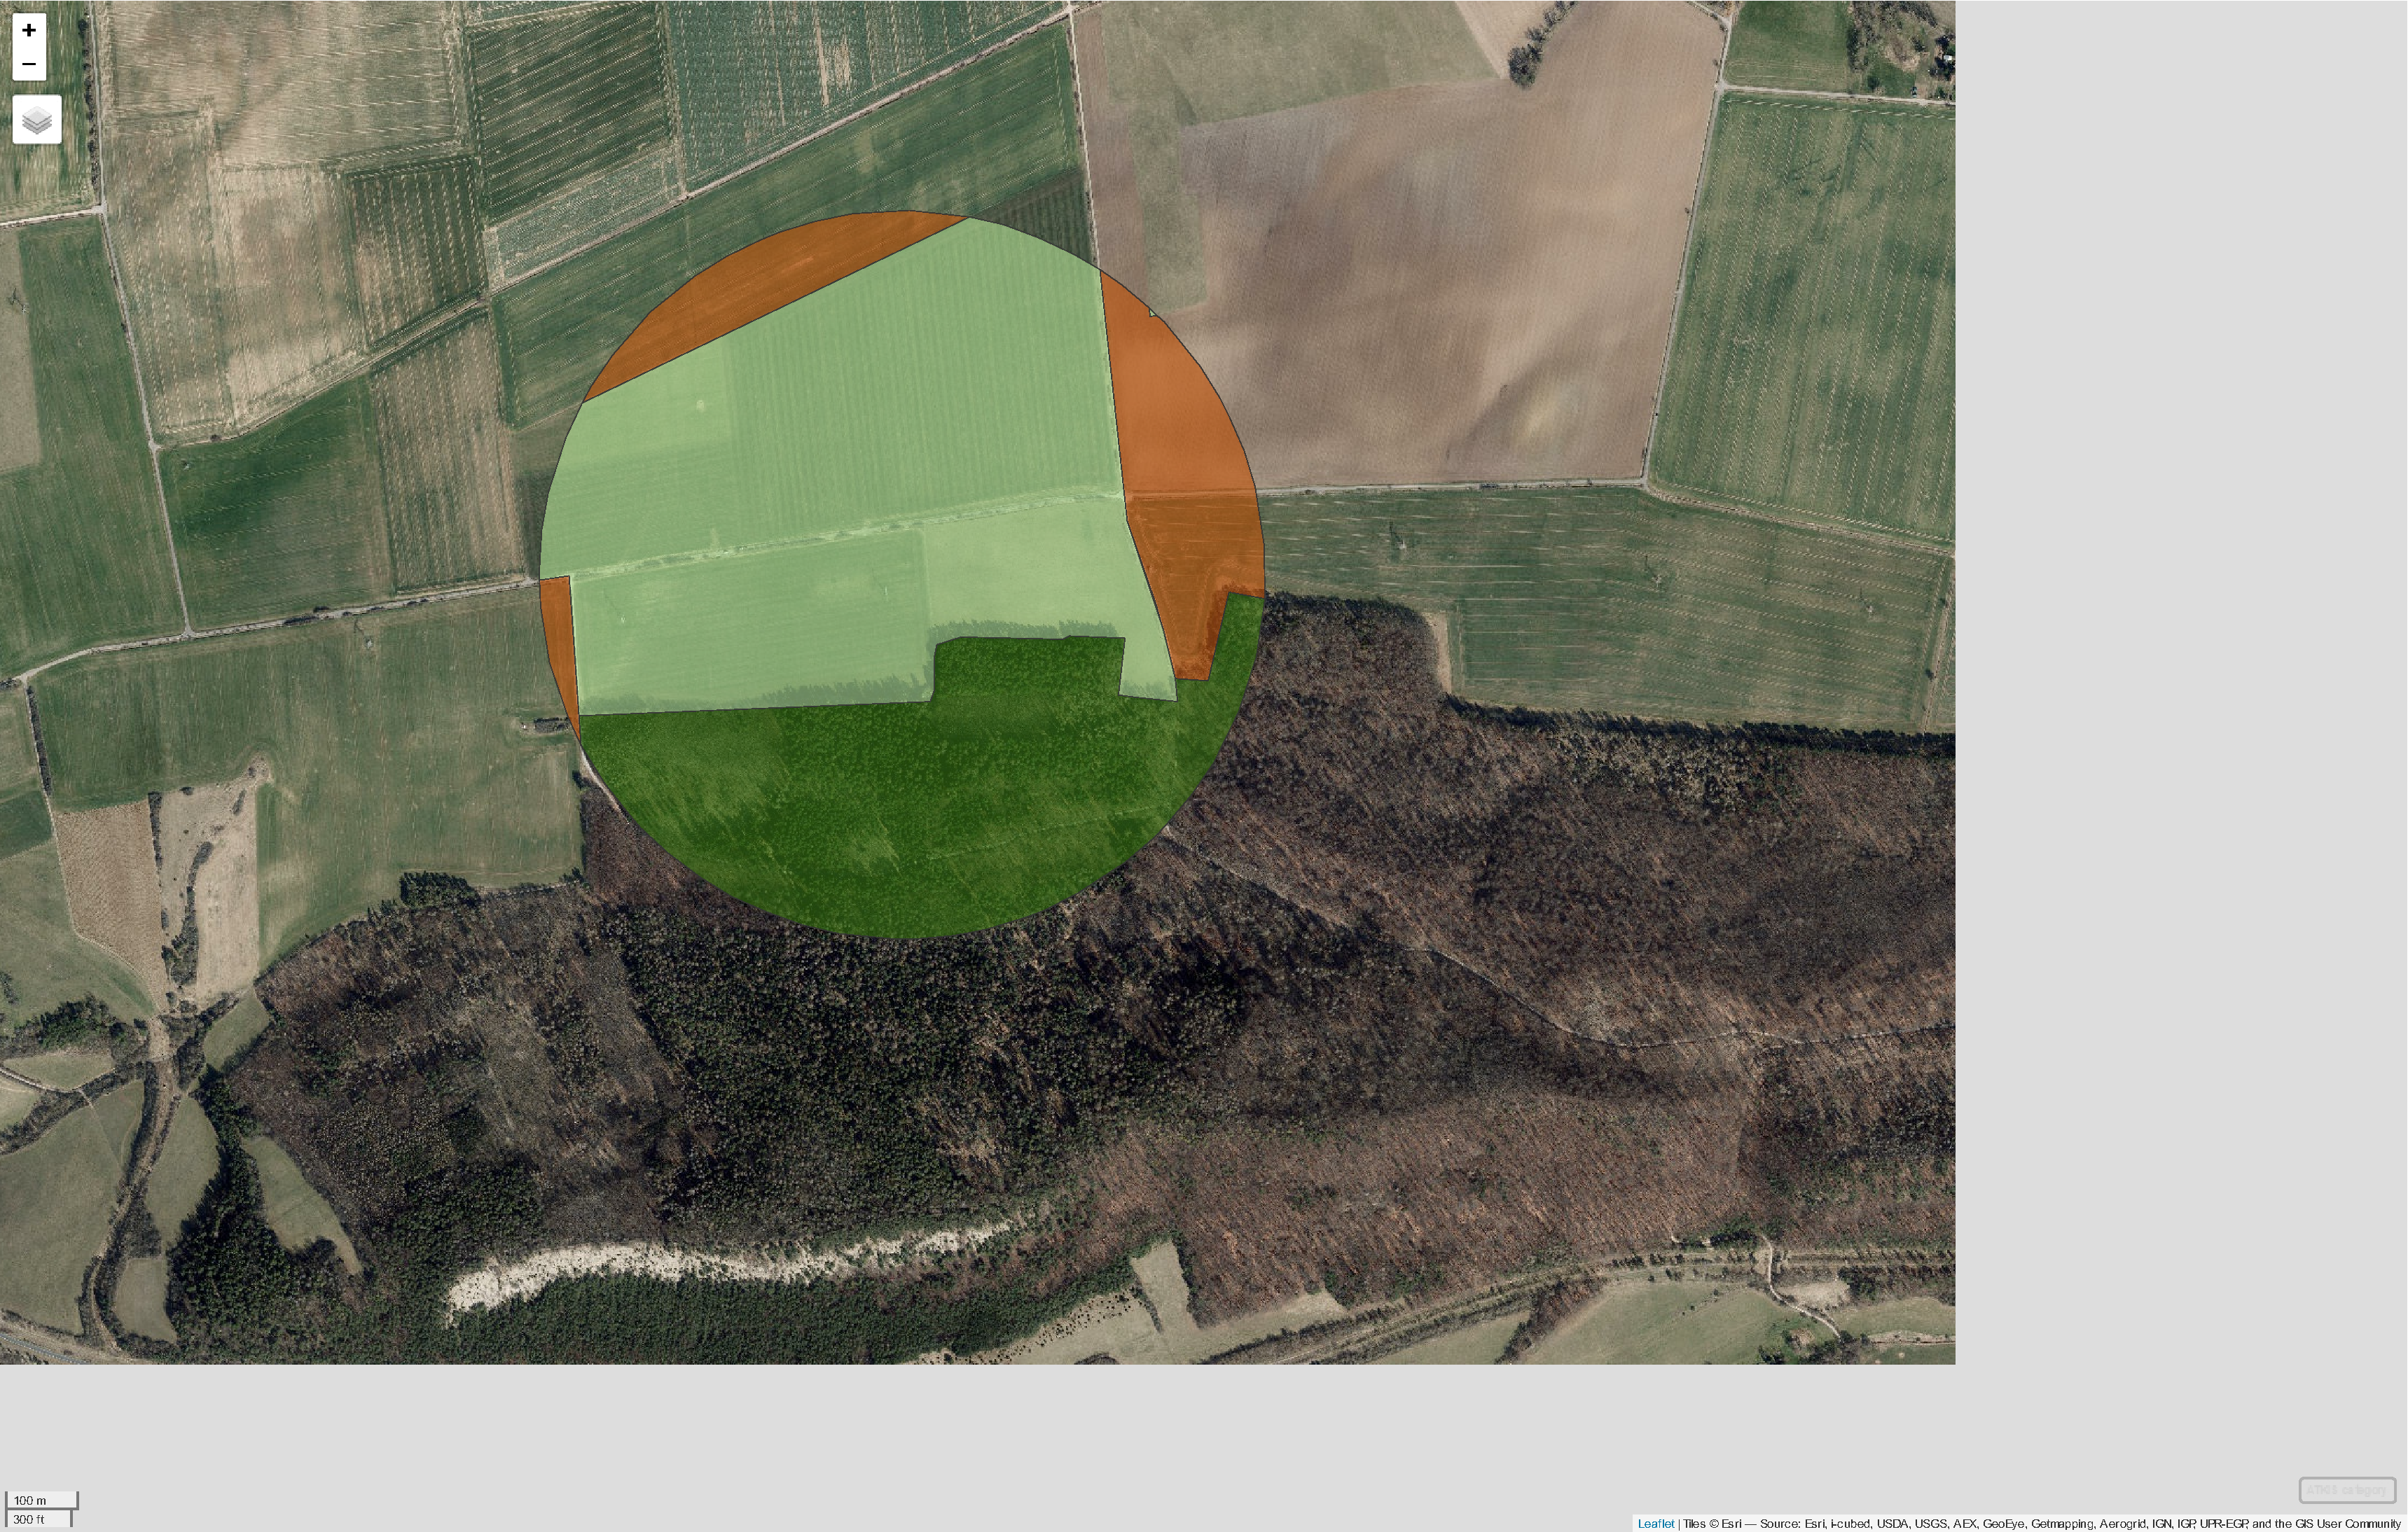
\includegraphics{Landscape_Indices_files/figure-pdf/unnamed-chunk-16-1.pdf}

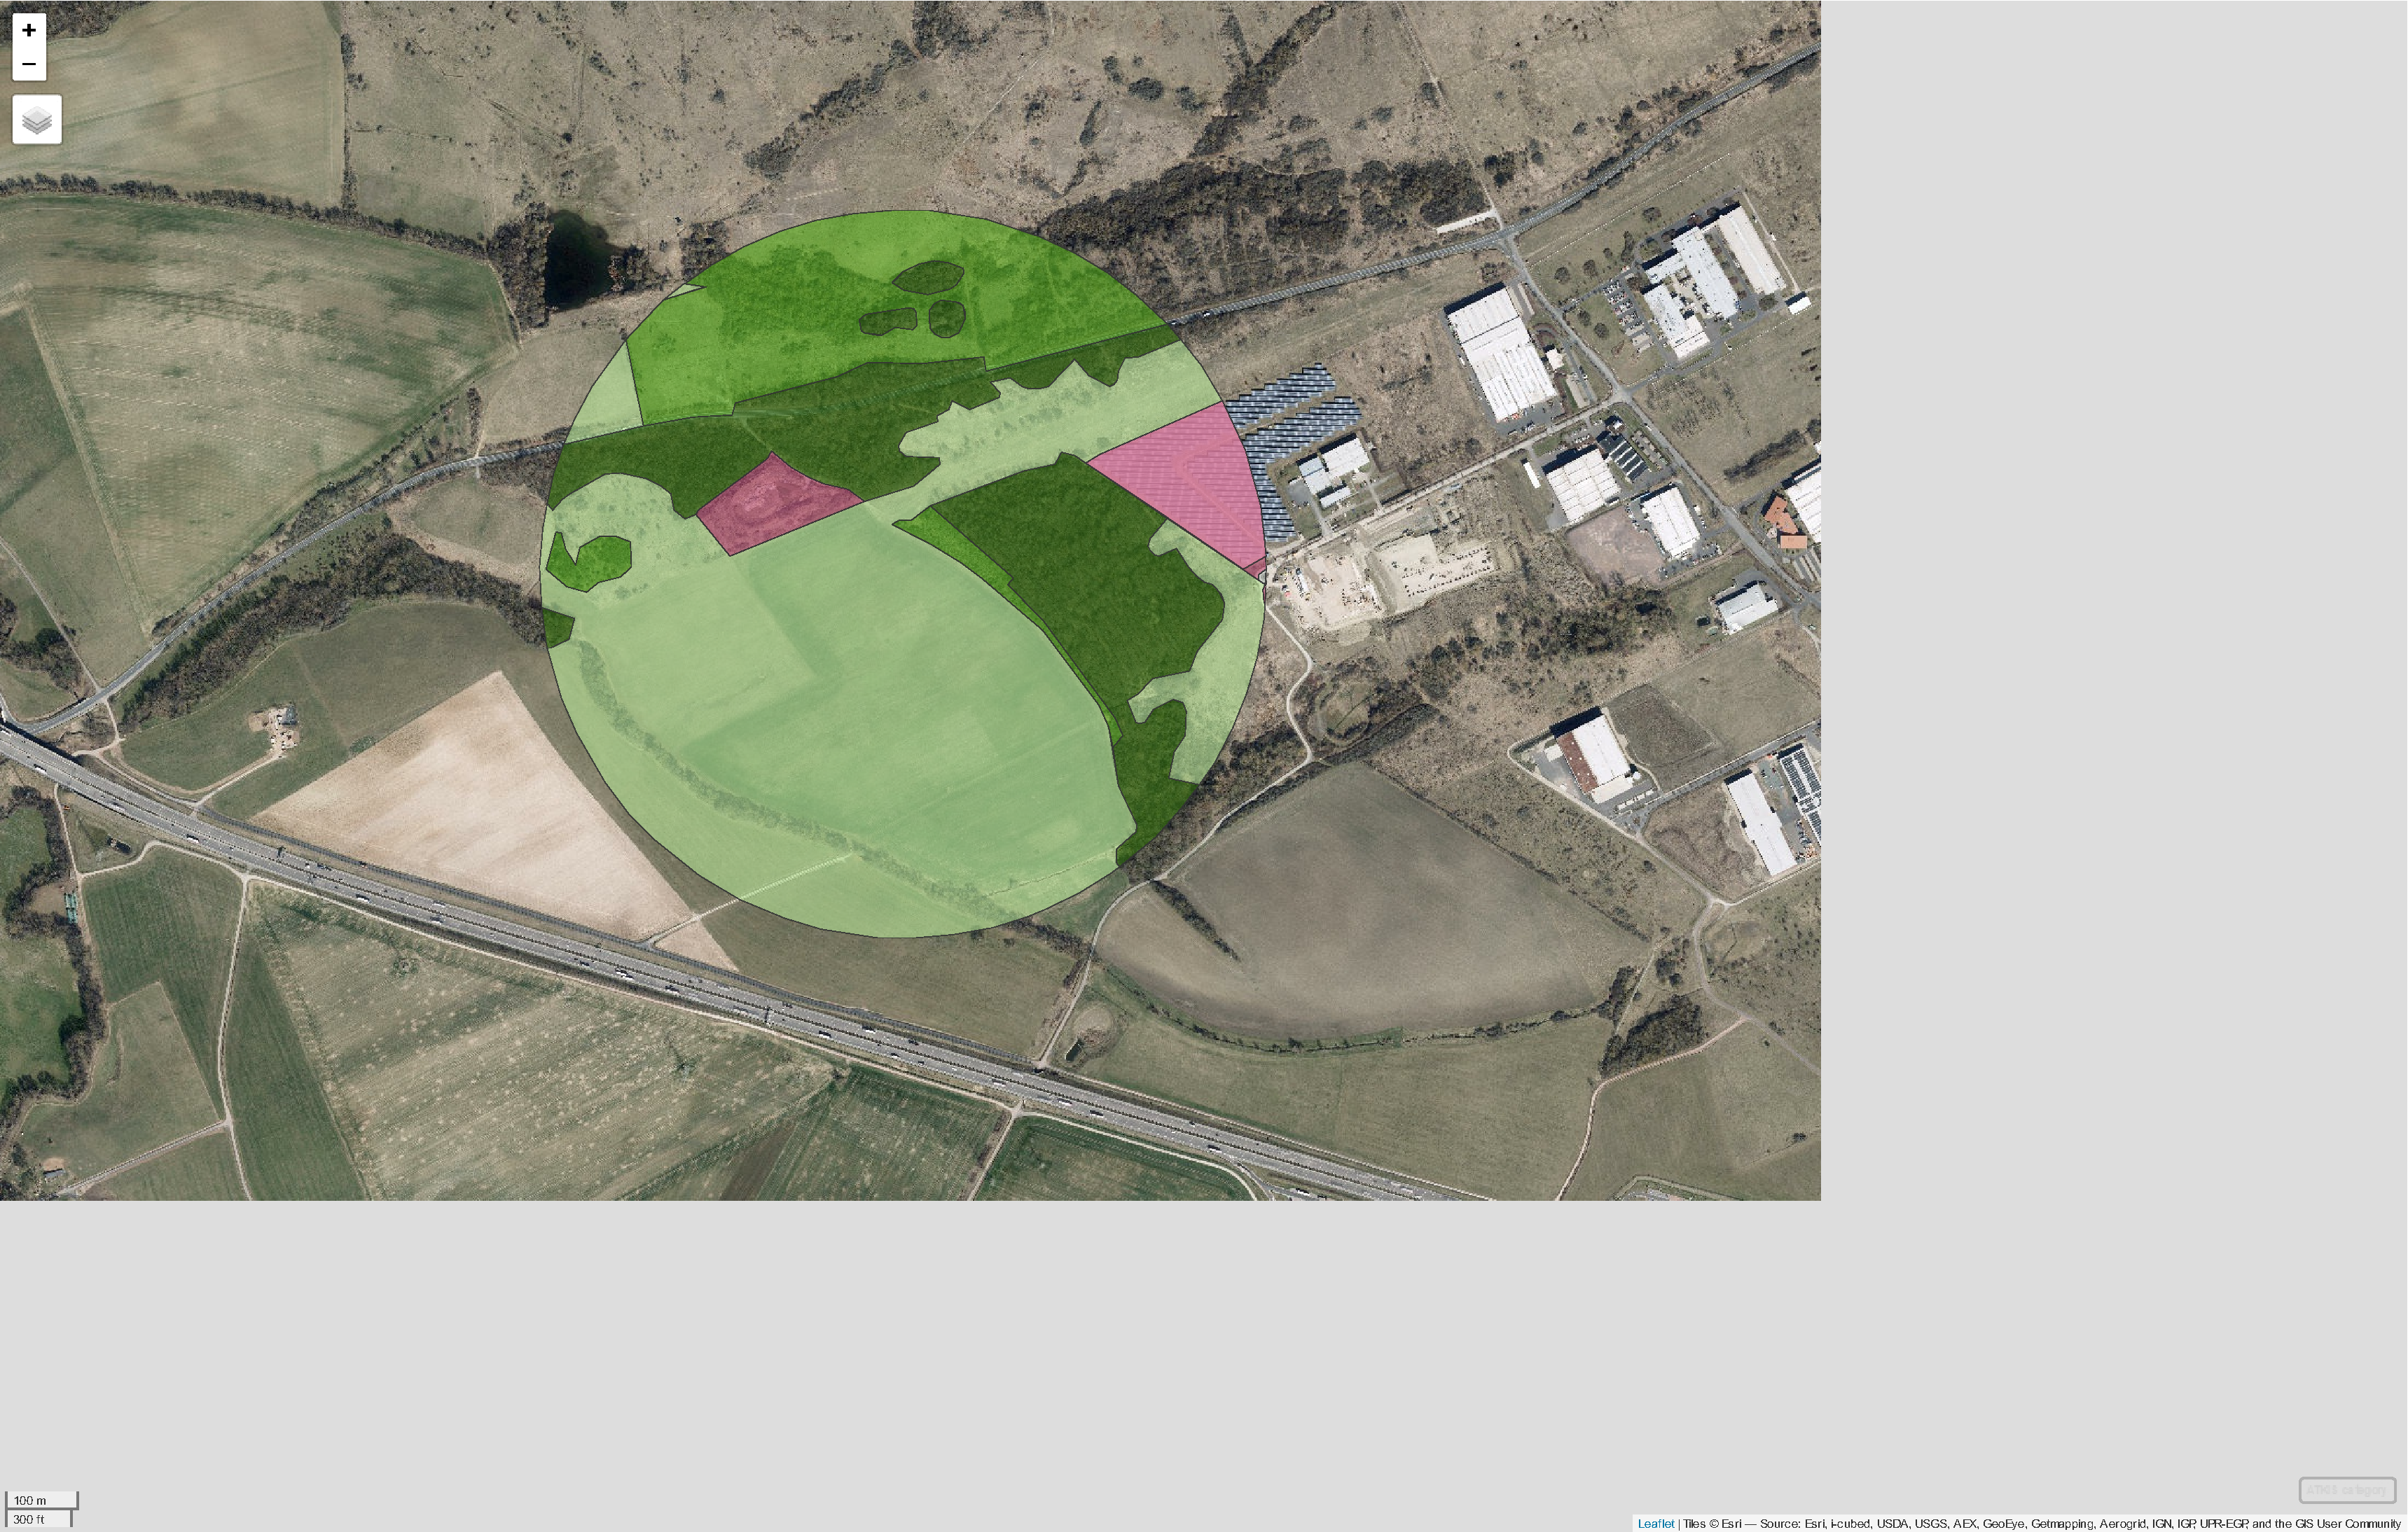
\includegraphics{Landscape_Indices_files/figure-pdf/unnamed-chunk-16-2.pdf}

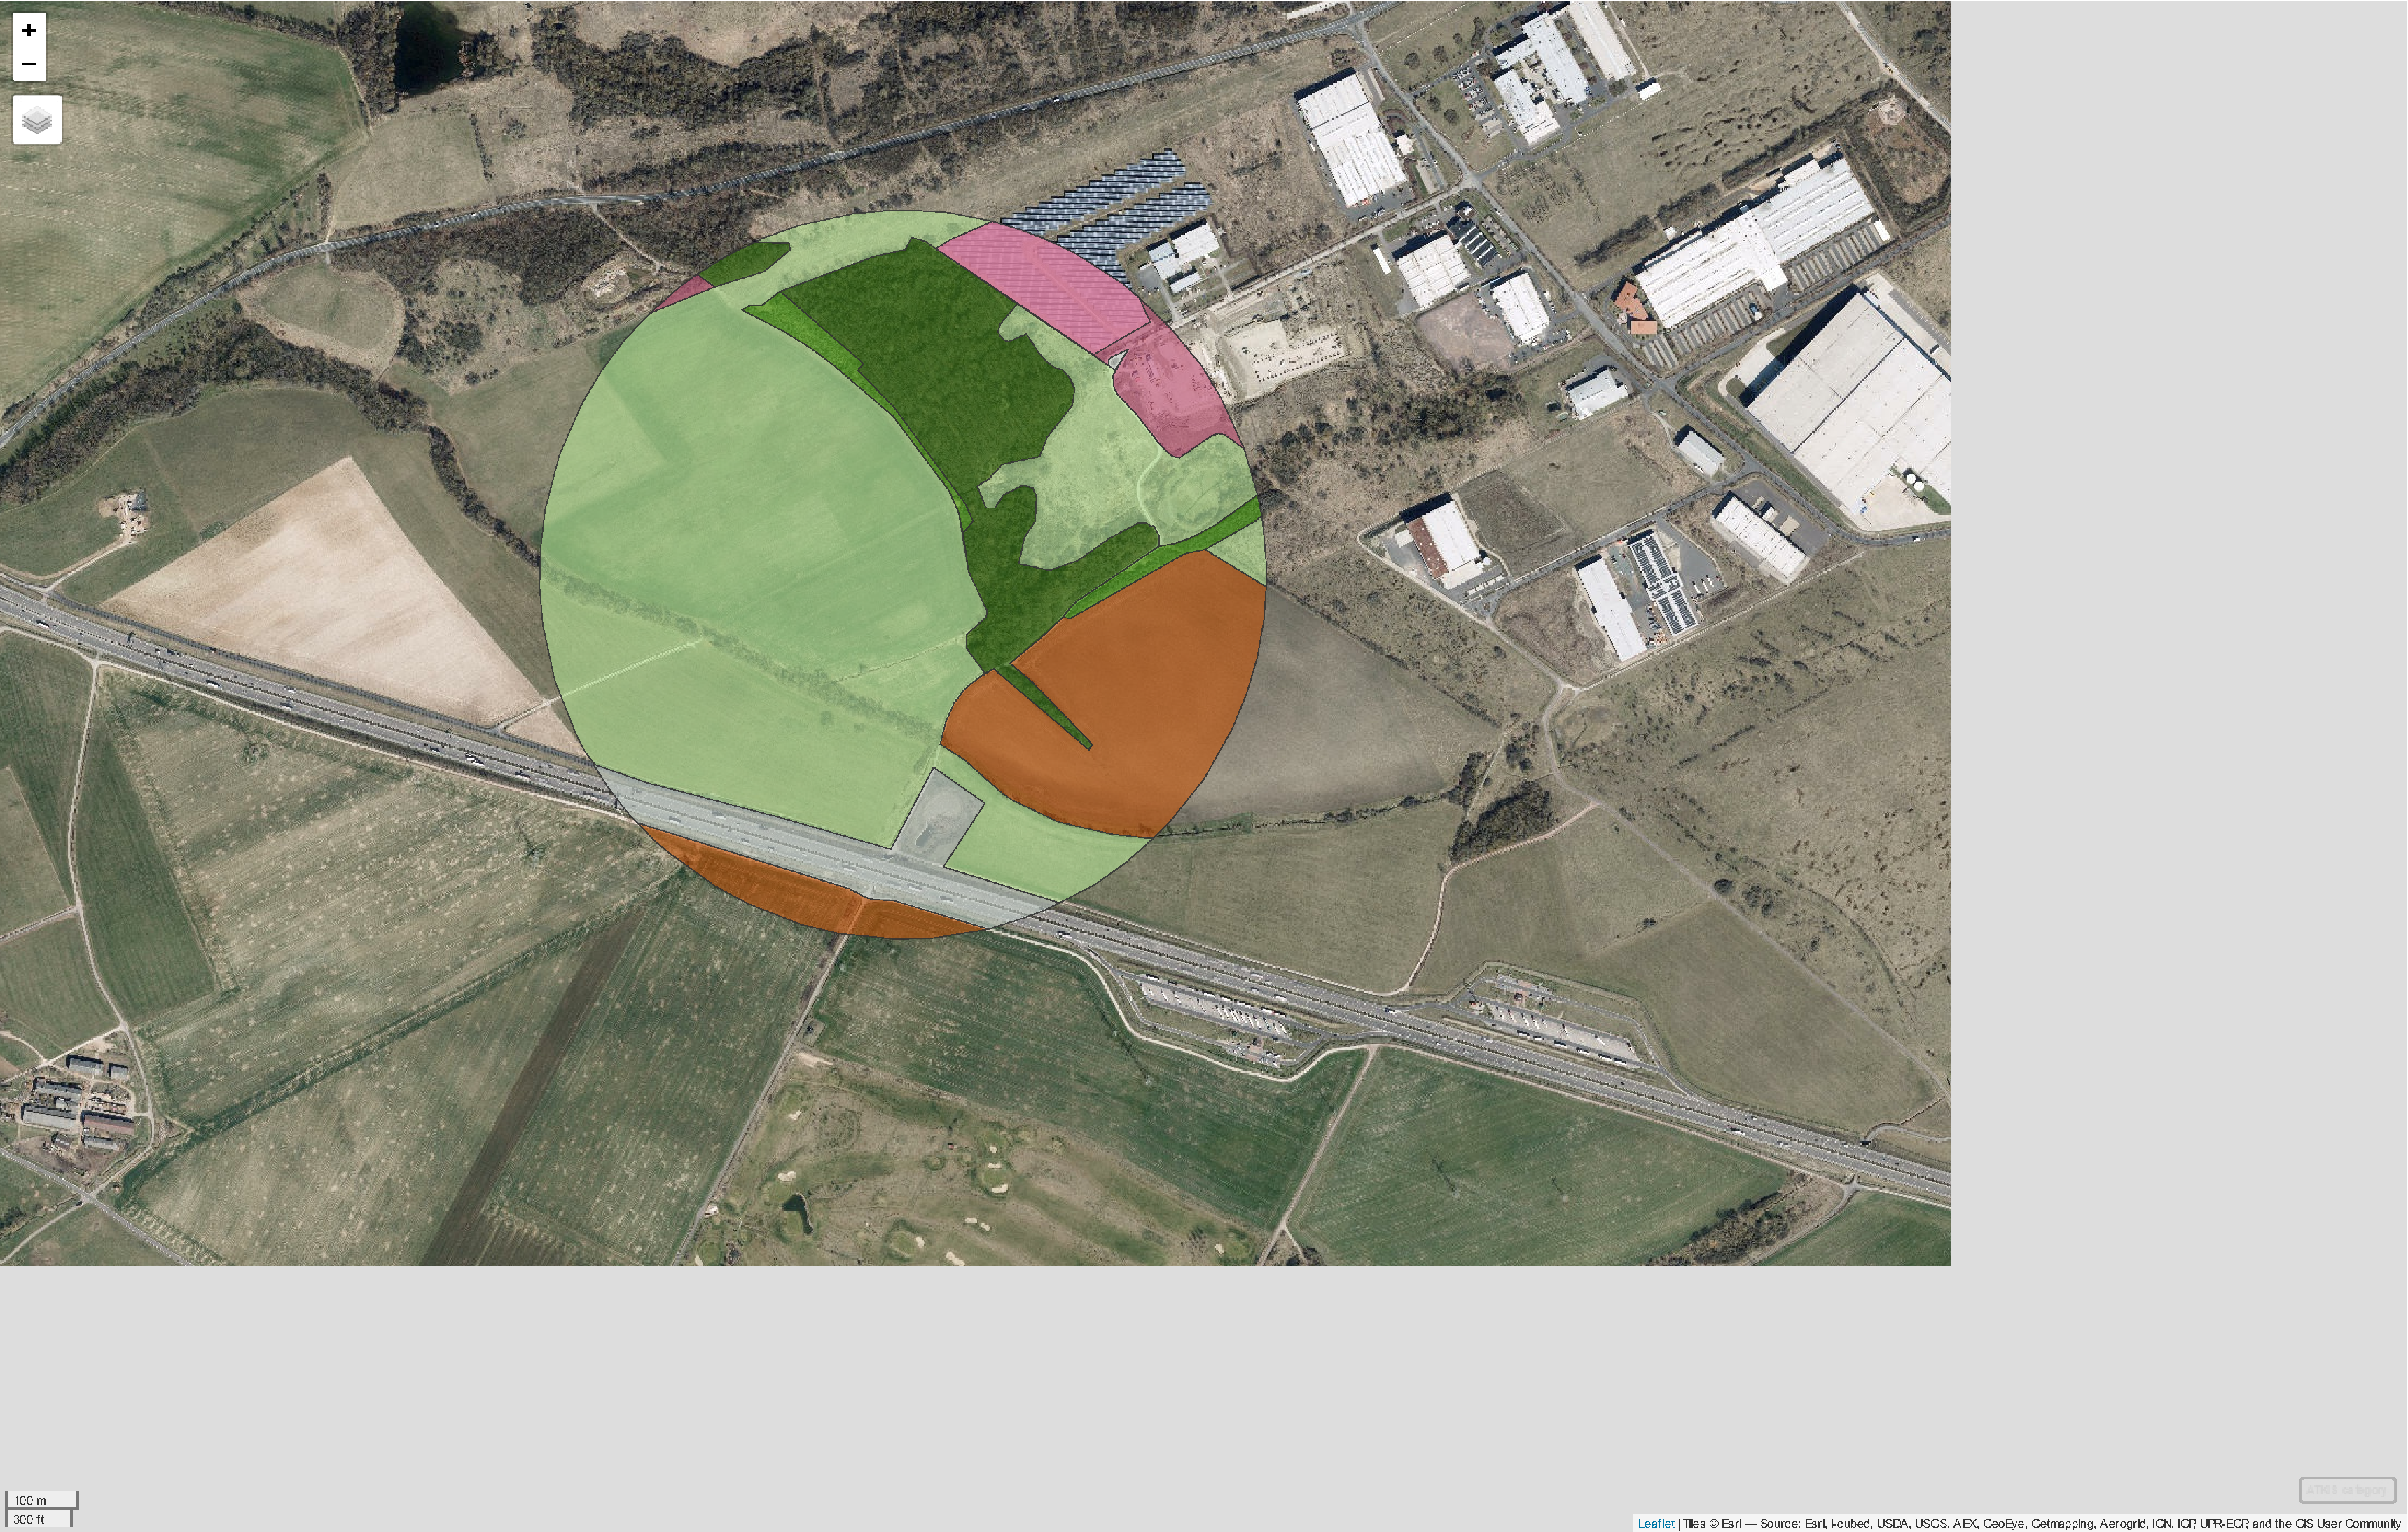
\includegraphics{Landscape_Indices_files/figure-pdf/unnamed-chunk-16-3.pdf}

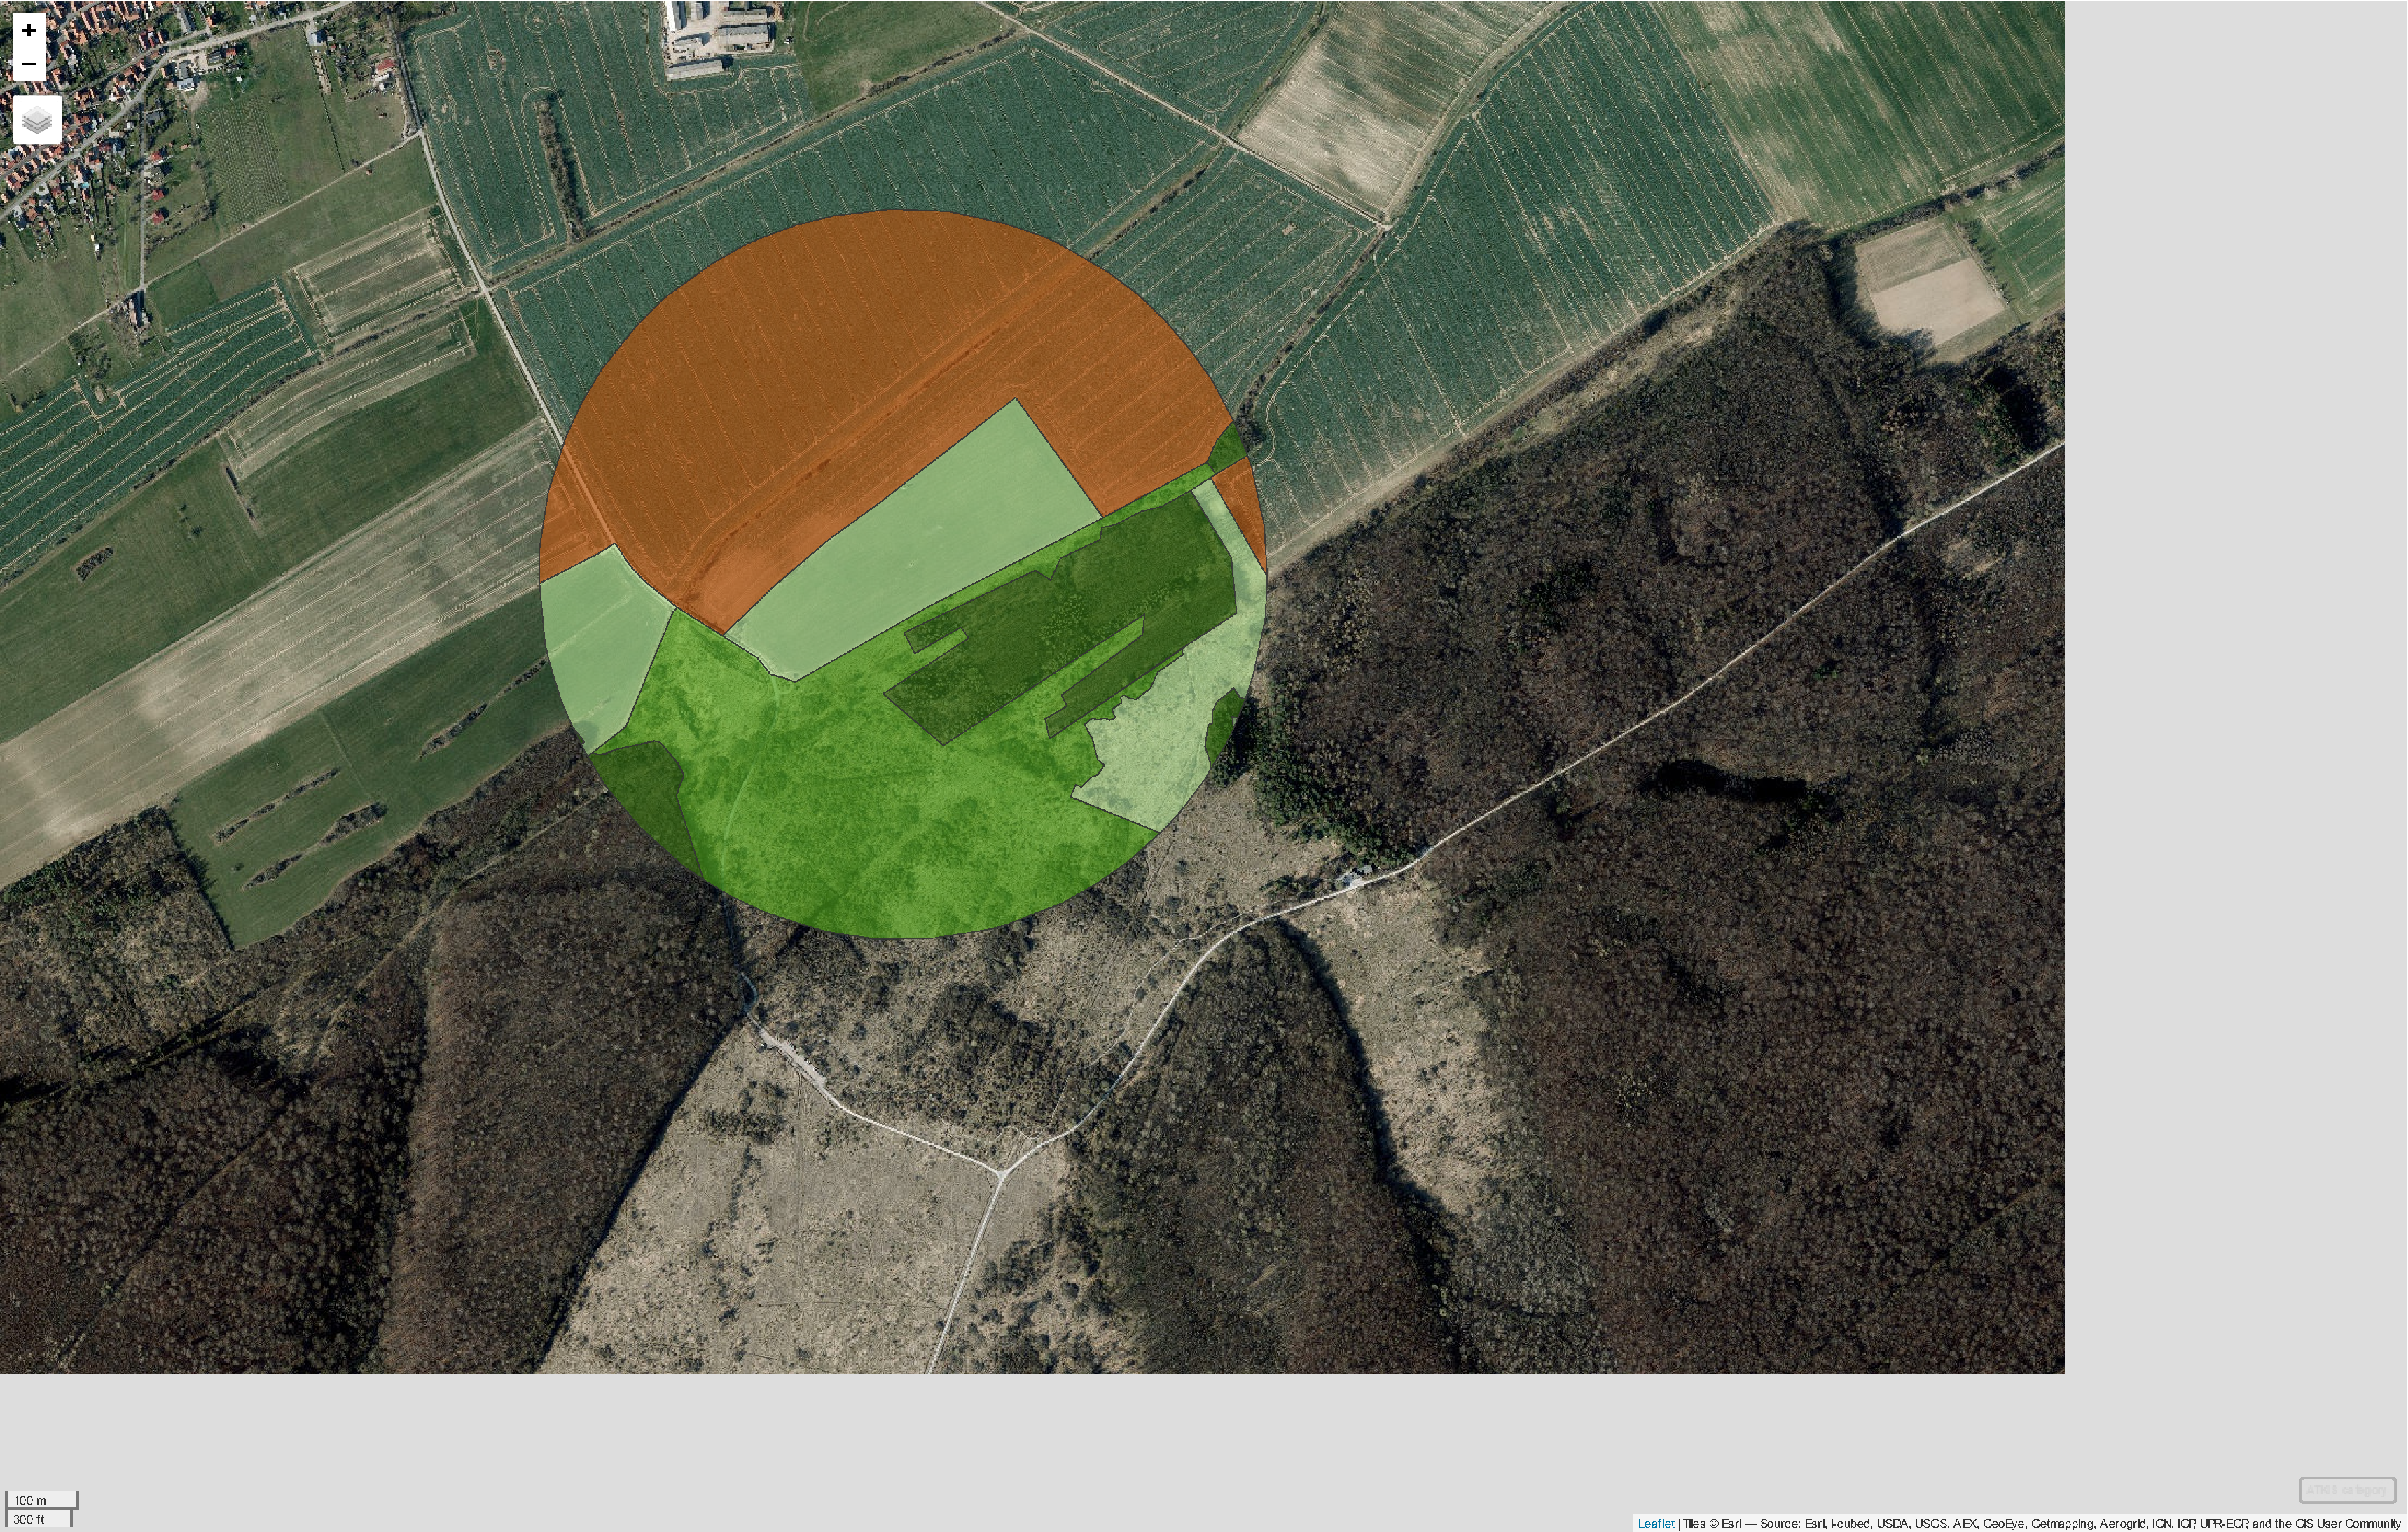
\includegraphics{Landscape_Indices_files/figure-pdf/unnamed-chunk-16-4.pdf}

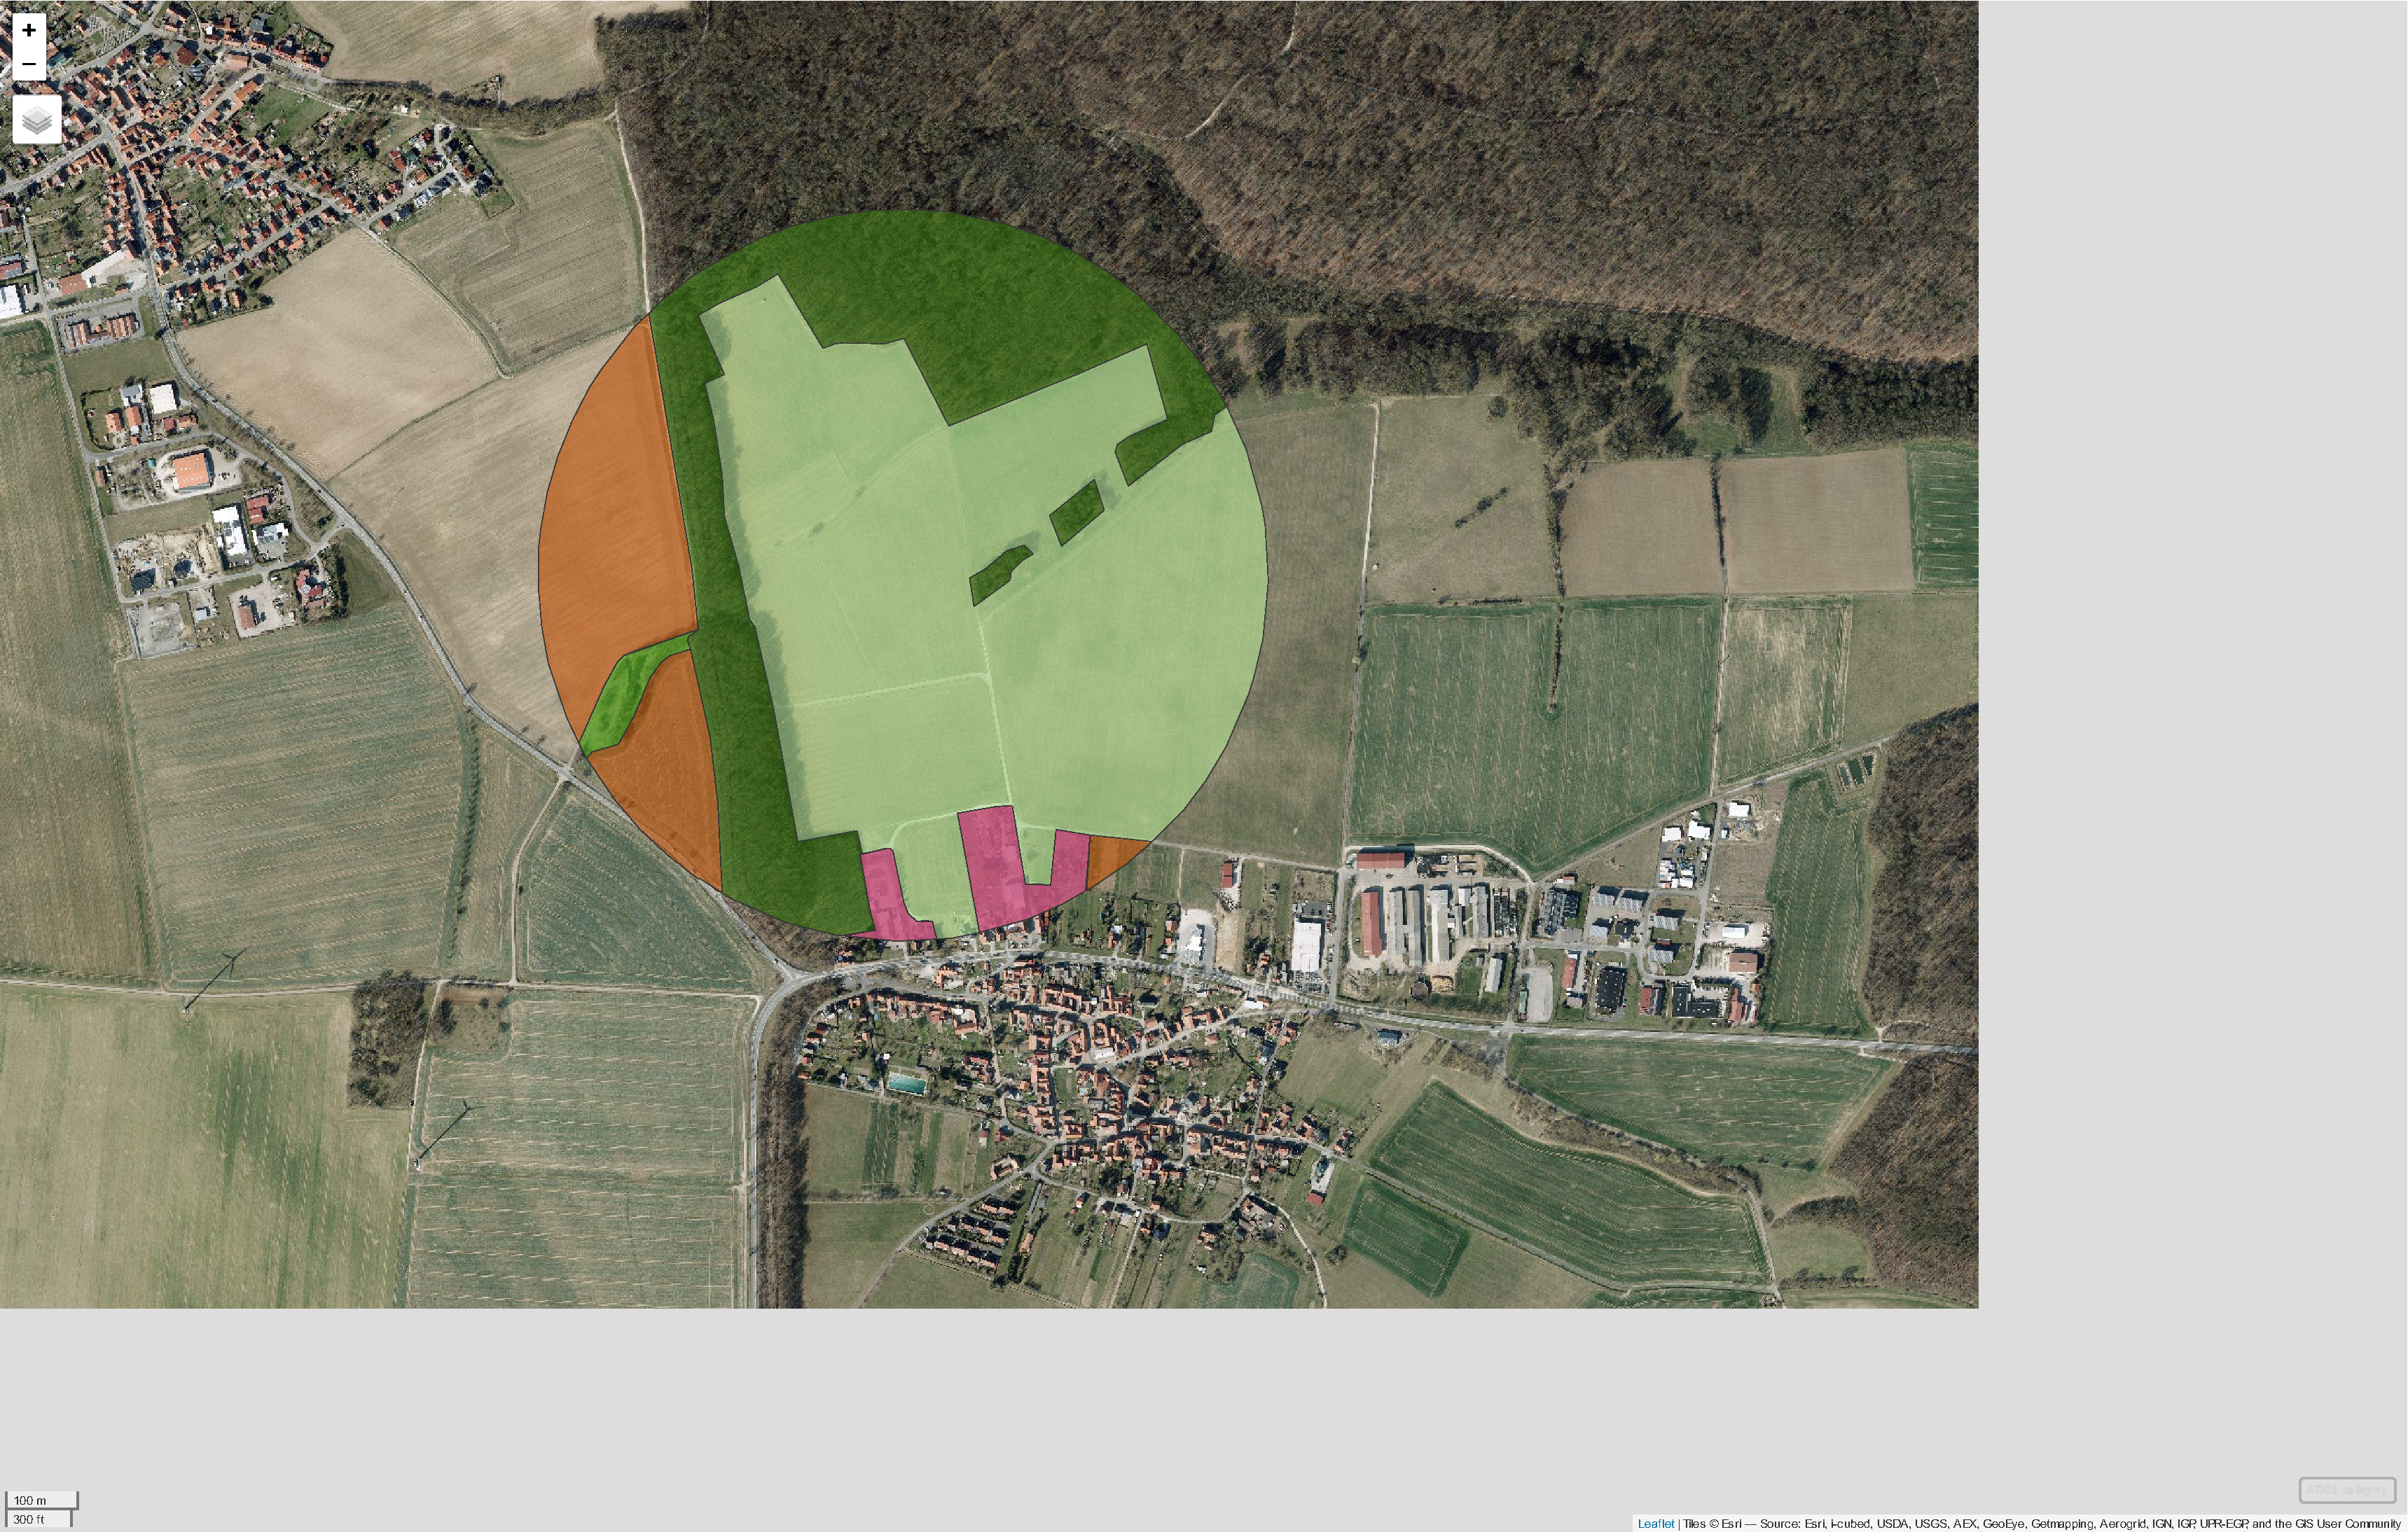
\includegraphics{Landscape_Indices_files/figure-pdf/unnamed-chunk-16-5.pdf}

Biodiversity and land use composition in the surrounding buffer:

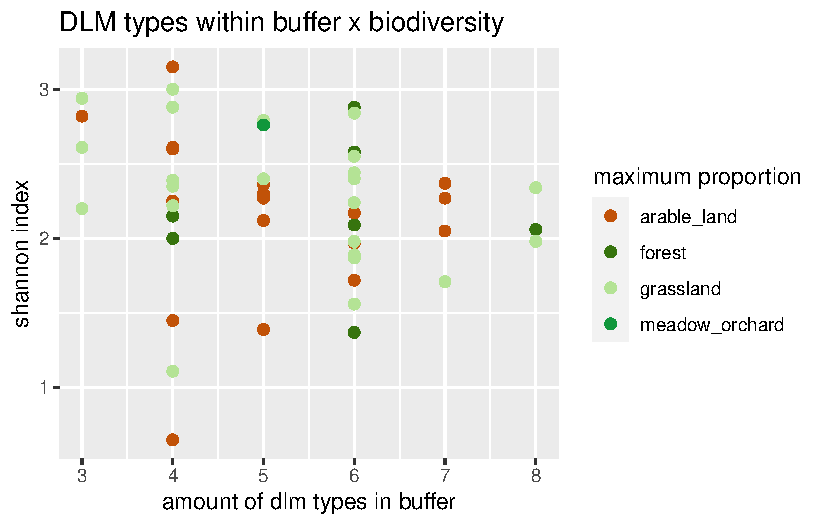
\includegraphics{Landscape_Indices_files/figure-pdf/unnamed-chunk-17-1.pdf}

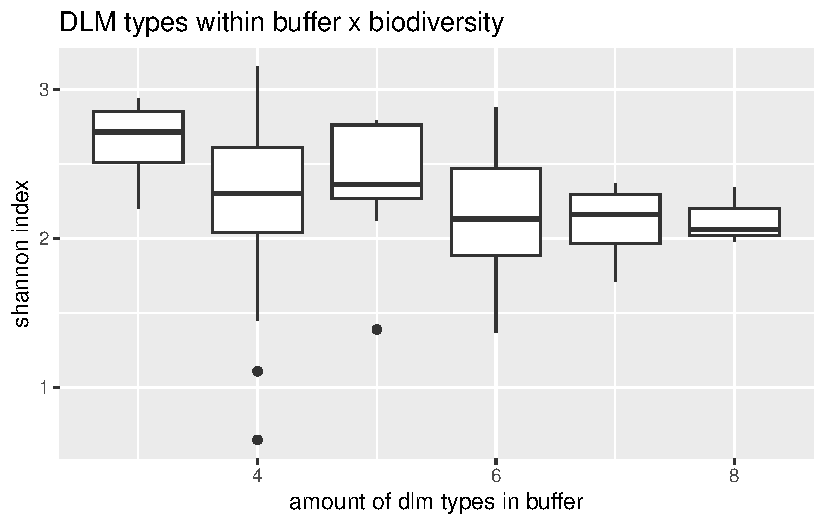
\includegraphics{Landscape_Indices_files/figure-pdf/unnamed-chunk-17-2.pdf}

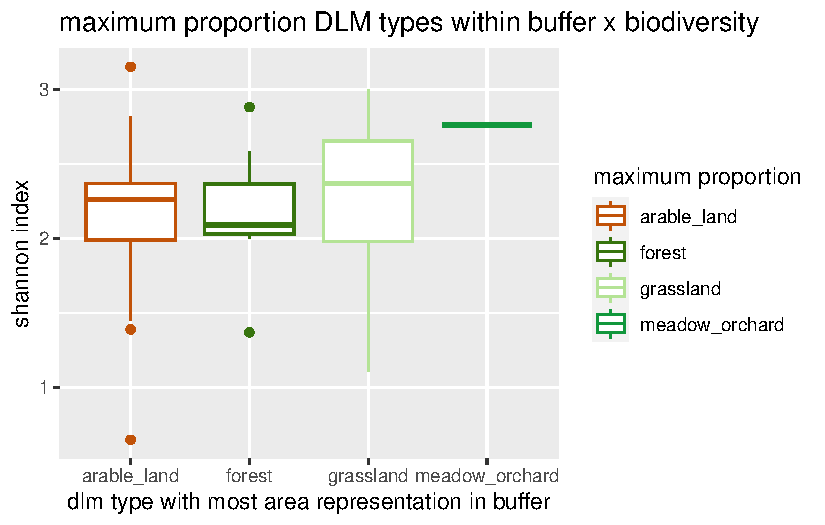
\includegraphics{Landscape_Indices_files/figure-pdf/unnamed-chunk-17-3.pdf}

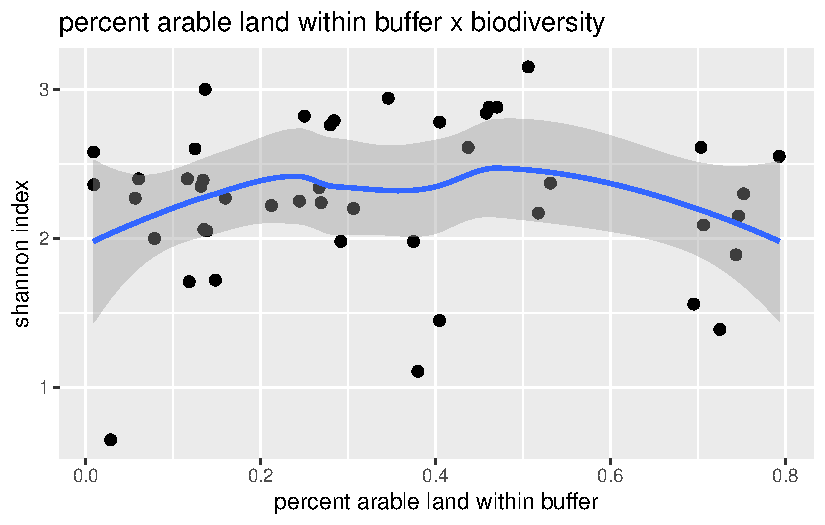
\includegraphics{Landscape_Indices_files/figure-pdf/unnamed-chunk-17-4.pdf}

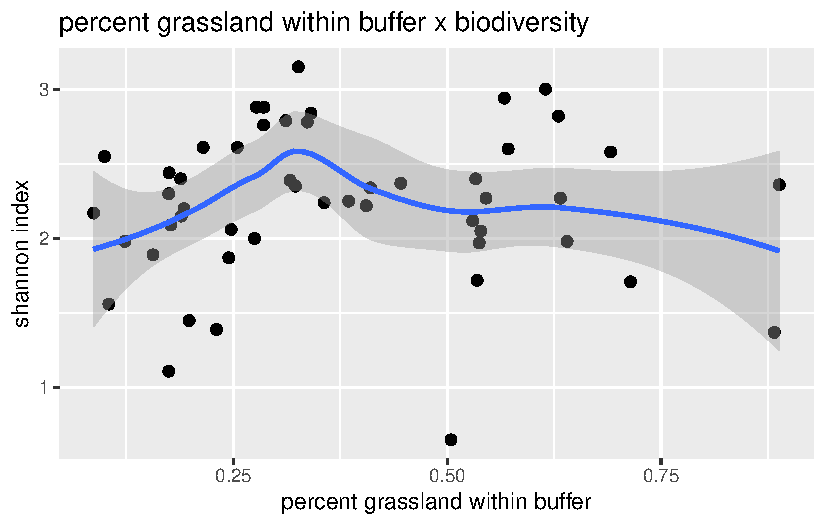
\includegraphics{Landscape_Indices_files/figure-pdf/unnamed-chunk-17-5.pdf}

\hypertarget{patch-metrics}{%
\subsection{Patch metrics}\label{patch-metrics}}

\begin{figure}

\begin{minipage}[t]{0.50\linewidth}

{\centering 

\raisebox{-\height}{

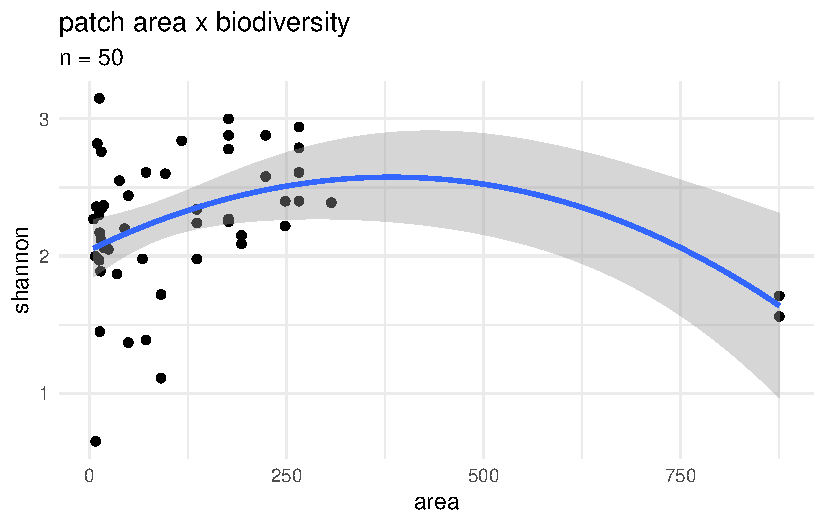
\includegraphics{Landscape_Indices_files/figure-pdf/unnamed-chunk-19-1.pdf}

}

}

\end{minipage}%
%
\begin{minipage}[t]{0.50\linewidth}

{\centering 

\raisebox{-\height}{

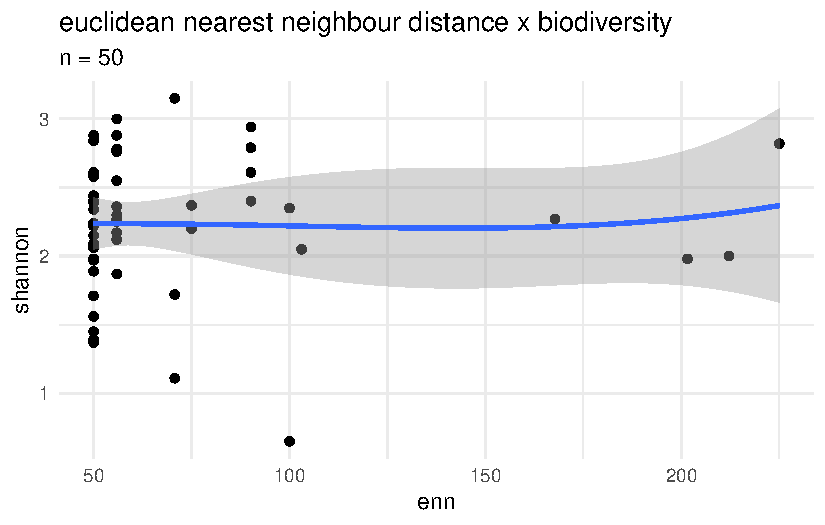
\includegraphics{Landscape_Indices_files/figure-pdf/unnamed-chunk-19-2.pdf}

}

}

\end{minipage}%
\newline
\begin{minipage}[t]{0.50\linewidth}

{\centering 

\raisebox{-\height}{

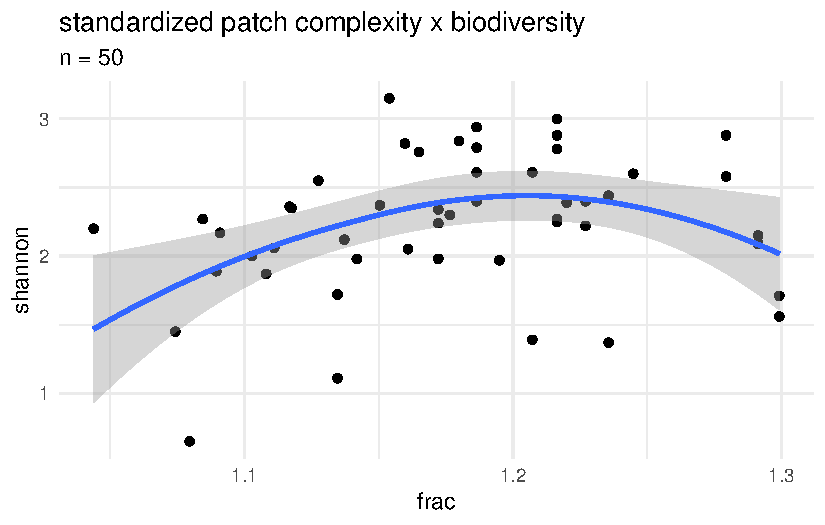
\includegraphics{Landscape_Indices_files/figure-pdf/unnamed-chunk-19-3.pdf}

}

}

\end{minipage}%
%
\begin{minipage}[t]{0.50\linewidth}

{\centering 

\raisebox{-\height}{

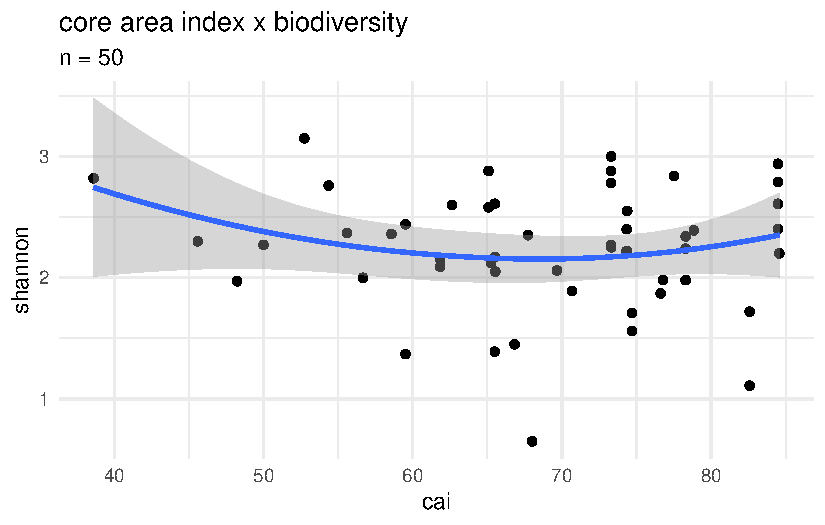
\includegraphics{Landscape_Indices_files/figure-pdf/unnamed-chunk-19-4.pdf}

}

}

\end{minipage}%

\end{figure}

\hypertarget{patch-shape-patch-complexity-distances-between-patches}{%
\subsubsection{\texorpdfstring{\textbf{Patch shape, Patch complexity,
distances between
patches}}{Patch shape, Patch complexity, distances between patches}}\label{patch-shape-patch-complexity-distances-between-patches}}

See calc\_patch\_metrics scripts trying landscapemetrics package and RS
Github Repo

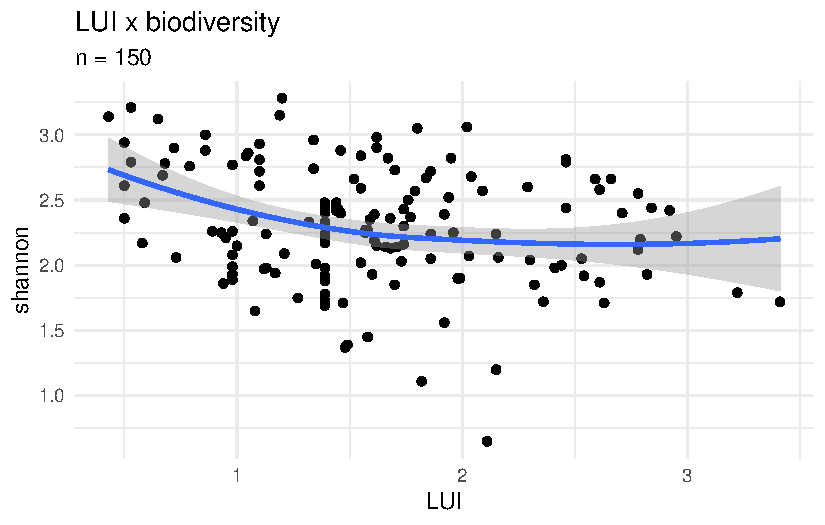
\includegraphics{Landscape_Indices_files/figure-pdf/unnamed-chunk-20-1.pdf}

\begin{figure}

\begin{minipage}[t]{0.33\linewidth}

{\centering 

\raisebox{-\height}{

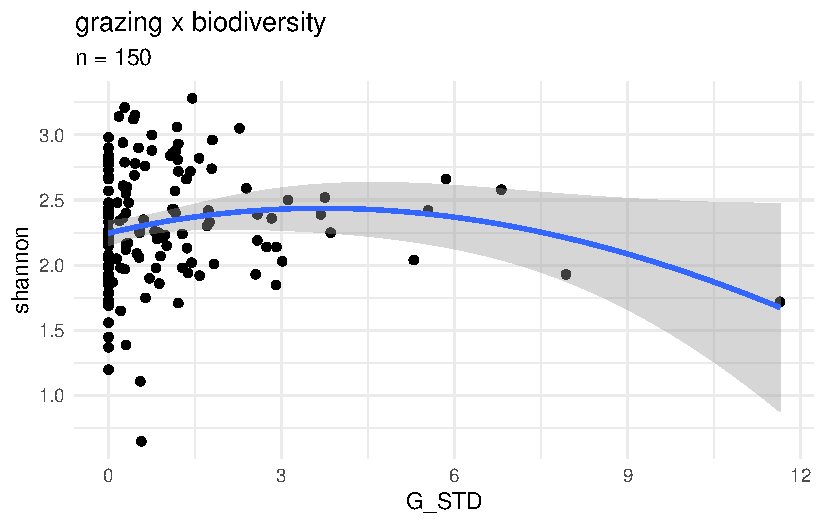
\includegraphics{Landscape_Indices_files/figure-pdf/unnamed-chunk-21-1.pdf}

}

}

\end{minipage}%
%
\begin{minipage}[t]{0.33\linewidth}

{\centering 

\raisebox{-\height}{

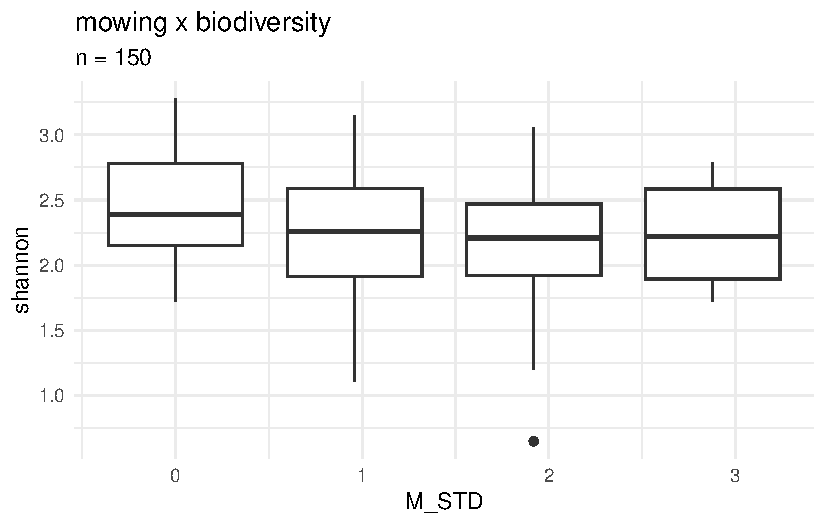
\includegraphics{Landscape_Indices_files/figure-pdf/unnamed-chunk-21-2.pdf}

}

}

\end{minipage}%
%
\begin{minipage}[t]{0.33\linewidth}

{\centering 

\raisebox{-\height}{

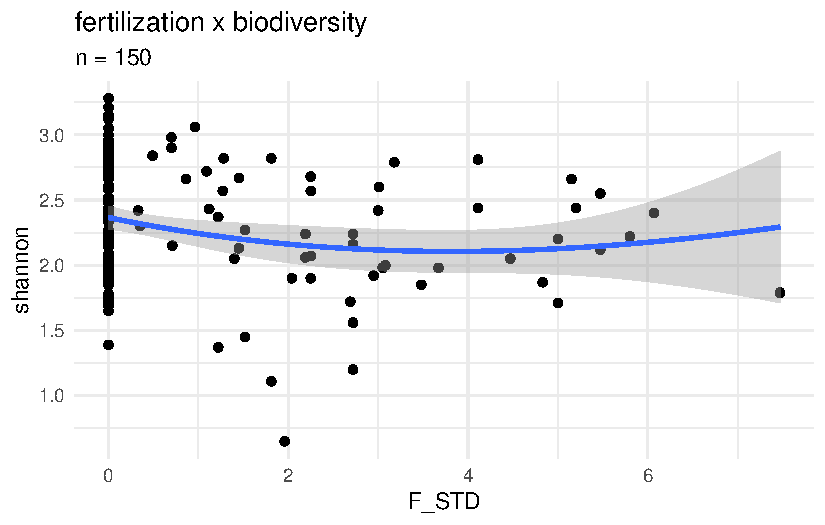
\includegraphics{Landscape_Indices_files/figure-pdf/unnamed-chunk-21-3.pdf}

}

}

\end{minipage}%

\end{figure}

There seems to be a statistical relation but at least for 2013 it seems
like the smaller the LUI the higher the diversity or even like
intermediate disturbances lead to lowest biodiversity\ldots{}

Hypothesis of highest biodiversity with intermediate disturbances seems
to be valid only for grazing (which makes sense given the further
explanation of the H),

\hypertarget{overall-correlations-within-the-dataset-and-with-predictors-terrain}{%
\subsubsection{Overall correlations within the dataset and with
predictors (terrain,
\ldots)}\label{overall-correlations-within-the-dataset-and-with-predictors-terrain}}

\begin{verbatim}
\end{verbatim}

\hypertarget{sources}{%
\subsection{Sources:}\label{sources}}

https://gistbok.ucgis.org/bok-topics/landscape-metrics\#:\textasciitilde:text=Landscape\%20metrics\%E2\%80\%94also\%20known\%20as,within\%20a\%20defined\%20geographic\%20area.

\hypertarget{to-do}{%
\section{to do:}\label{to-do}}

Fließgewässer, stehende trennen, sonst versiegelte Fläche zusammenfassen



\end{document}
